\chapter{Non-manifold Embedding for Geometry and Contact}
\label{chp:nonmanifold}

\section{Non-manifold Embedding}
\label{sec:hybrid}

We employ an embedded simulation similar to other authors, who used
regular lattice embeddings for performance
~\citep{MuellTG:2004,RiverJ:2007,McAdaZSETTS:2011}. However, due to the
presence of extremely thin incisions common in surgical models, standard
lattice embedding would not be able to resolve the tissue topology,
unless an extremely high resolution embedding was used. We thus adopt
a non-manifold lattice-derived embedding discretization in the spirit
of Virtual Node or XFEM methods
~\citep{MolinBF:2004,SifakDF:2007,NesmeKJF:2009}.  In this chapter, we
describe how these non-manifold embedding structures can be easily
constructed and how they can be used for handling contact scenarios in
addition to geometry representation. The following chapter will
discuss how these structures can be further optimzed for parallel
processing.

\subsection{Surface Model}

\begin{figure}
  \centering
  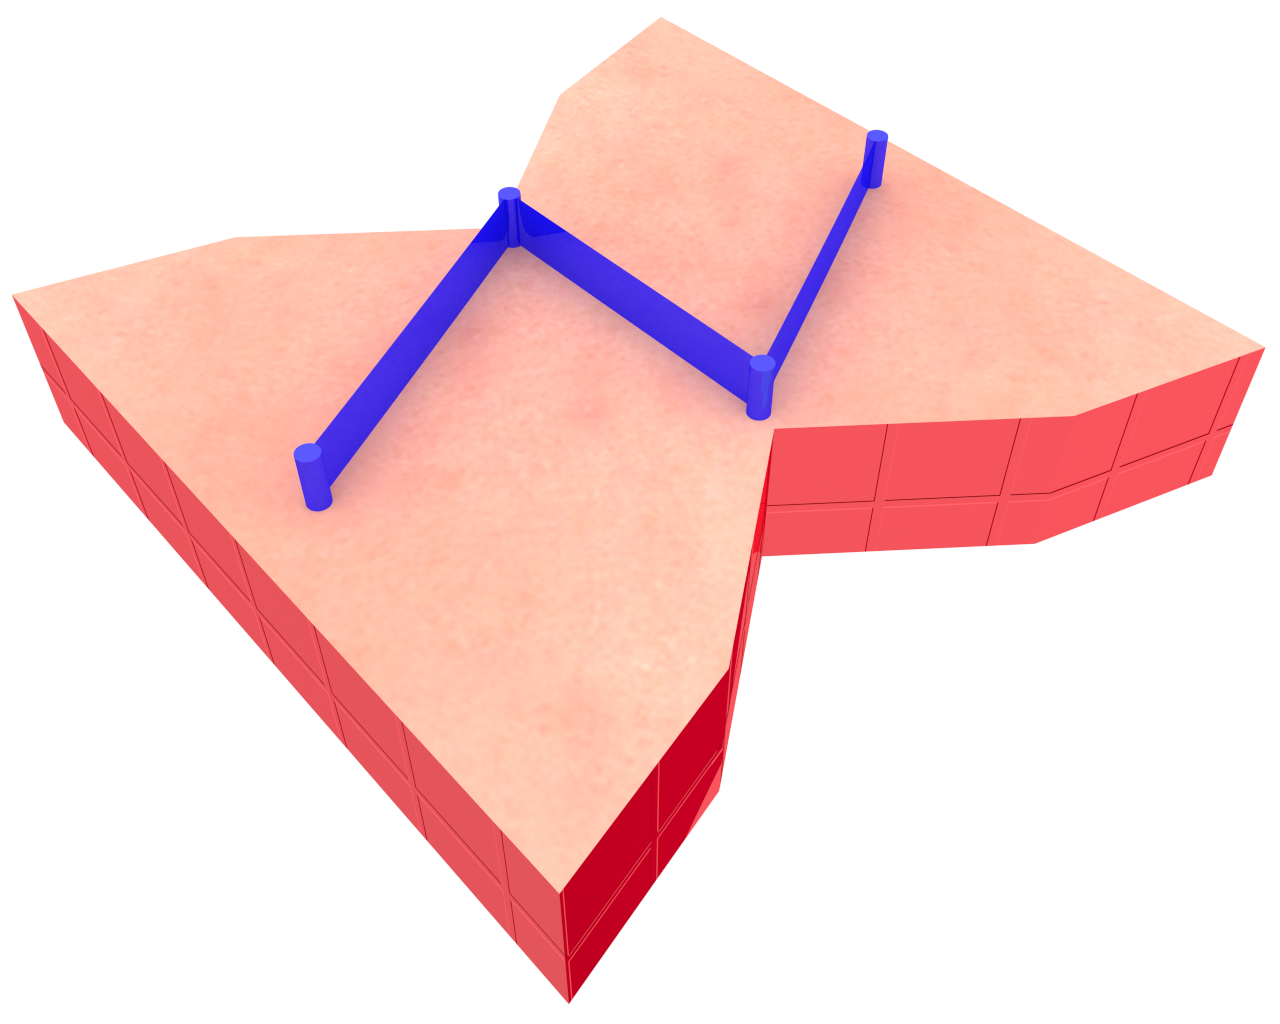
\includegraphics[width=.45\columnwidth]{chapter_gridiron/images/Uncut_Surface_Model2.png}
  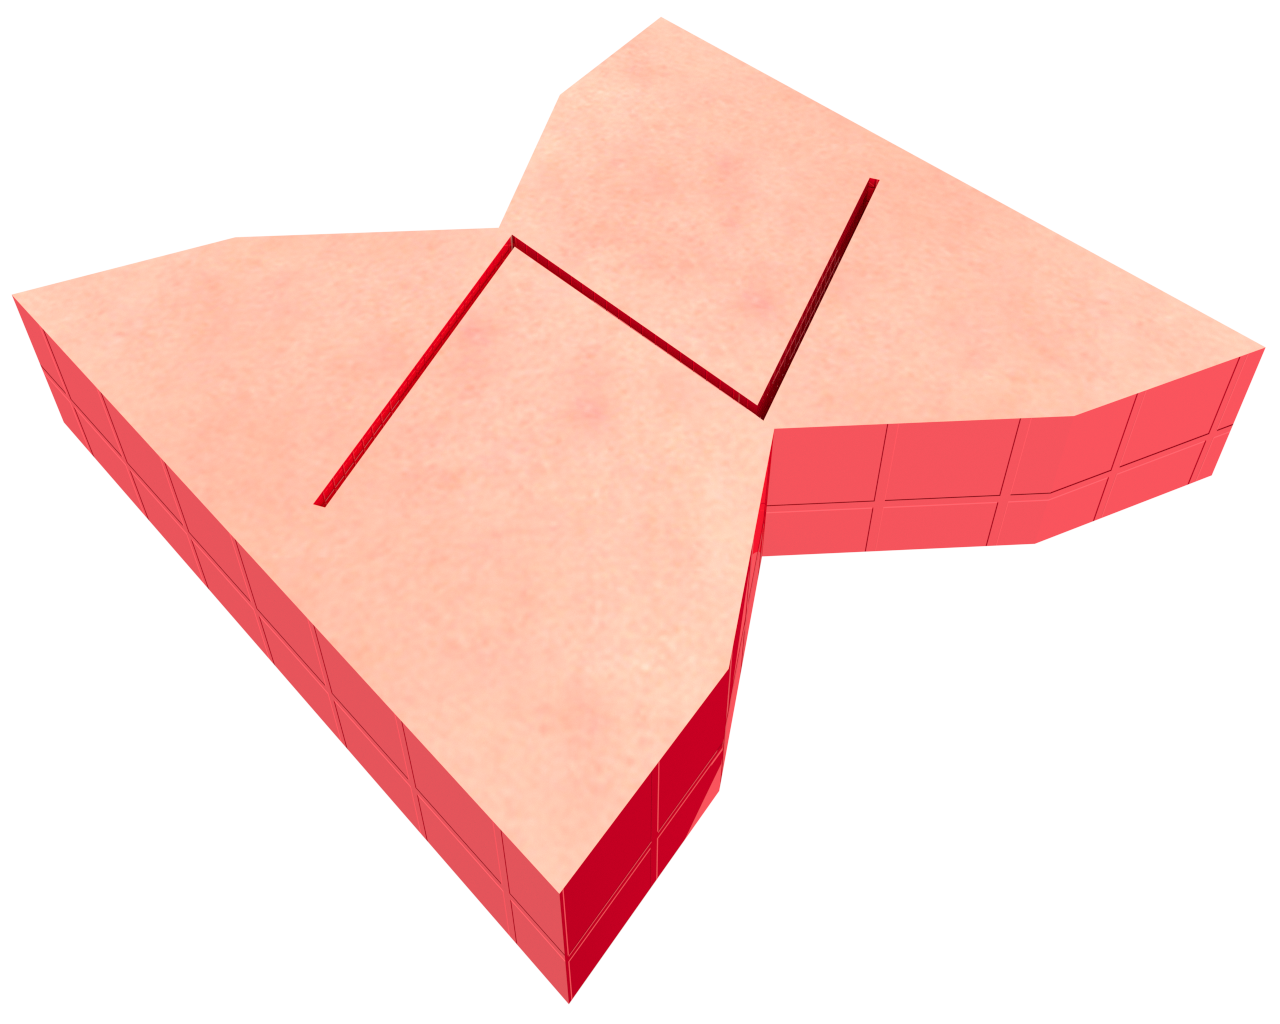
\includegraphics[width=.45\columnwidth]{chapter_gridiron/images/Cut_Surface_Model2.png}
  \caption{Illustration of incision technique}{Incisions in the flesh surface model are created by extruding and thickening user specified line segments.}
\label{fig:incision}
\end{figure}

Prior to elasticity discretization, a watertight surface model of the
flesh, including any incisions, must be created. The method choosen to
generate these models is immaterial to our embedding algorithm, but
for completeness we present our solution for incising surgical tissue
models. In our system, incisions are generated from user specified
line segment curves, which guide constructive solid geometry (CSG)
difference operations to produce cut surface meshes.  We begin from a
user specified line segment curve from which we construct prisms by
thickening the line segments tangentially and perpendicularly along
the surface normal. We then apply these prisms in a subtraction
operation with the surface, resulting in a slightly thickened incision
(Figure \ref{fig:incision}). Disconnected regions produced during this
step can be marked and removed by the user. Note that for scenarios
involving malignant tissue, discarding of excised tissue is
commonplace.

\subsection{Rasterization}

\begin{figure}
  \centering
  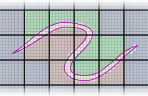
\includegraphics[width=\columnwidth]{chapter_gridiron/images/Figure_Topology_C}
  \caption{Illustration of the fine grid rasterization of a cut}{Fine cells within the cut are empty, and colored to show material continuity.}
\label{Fig:CuttingFineGrid}
\end{figure}


\begin{algorithm}
  \caption{Non-Manifold Simulation Mesh Construction}{This algorithm
    describes the steps required to identify material connectivity
    across voxel boundaries, and generate appropriate voxel topologies
    which respect this underlying material toplogy. Material
    continuity across voxel faces results in vertex collapse. While
    this can lead to loss of simulation resolution near incision
    points, it doesn't affect the embedding process and is less
    complicated to simulate. }
\label{alg:NonmanifoldMeshGeneration}
\begin{algorithmic}[1]
\Require Coarse Resolution
\Function{Generate$\_$Nonmanifold$\_$Mesh}{}

  \ForAll{Coarse Cells: $i$}
     \State $C$ $\gets$ \Call{Determine$\_$Material$\_$Components}{$i$}
     \ForAll{ Components in $C$ }
     \State Instance separate copy of $i$
     \State Generate unique, separate DOFs
     \State Assign descriptor of material content
  \EndFor
\EndFor

   \ForAll{Geometrically adjacent cell pairs: $(i, j)$}
      \ForAll{Pairs of duplicates from $i$ and $j$: $(h, k)$}
         \If{ \Call{Material$\_$Is$\_$Continuous}{$h$, $k$} }
            \State Mark shared vertices as equivalent
         \EndIf
      \EndFor
   \EndFor

   \ForAll{Coarse Cells: $i$}
      \State Compare all duplicates of $i$
      \State Collapse duplicates with equivalent DOF's
   \EndFor
\EndFunction
\Ensure An explicit, possibly non-manifold mesh
\end{algorithmic}
\end{algorithm}


Given a cut surface mesh, we first create a fine rasterization of the
surface. The resolution of the rasterization is selected to capture
all desired topological detail (typically an order of magnitude finer
than simulation resolution). In Figure \ref{Fig:CuttingFineGrid}, it
is possible to see the fine rasterization grid in contrast to the
coarser simulation resolution.  The rasterization is performed by
detecting all voxels intersected by the object surface and
flood-filling to mark the volumetric material region.  Once the
rasterization is complete, subsequent embedding operations are purely
combinatorial and not sensitive to poor conditioning of surface mesh
elements.  Additionally, this fine-grid embedding can also act as an
interface layer to more complex embedding schemes, such as the
non-manifold approach described next. We leverage this by translating
any deformation results back to the fine-grid embedding prior to
rendering, to hide non-manifold embedding or numerical solution
details from the visual front-end.

\subsection{Non-Manifold mesh generation}
\label{sec:nonmanifoldmeshgeneration}

\begin{figure}
  \centering
  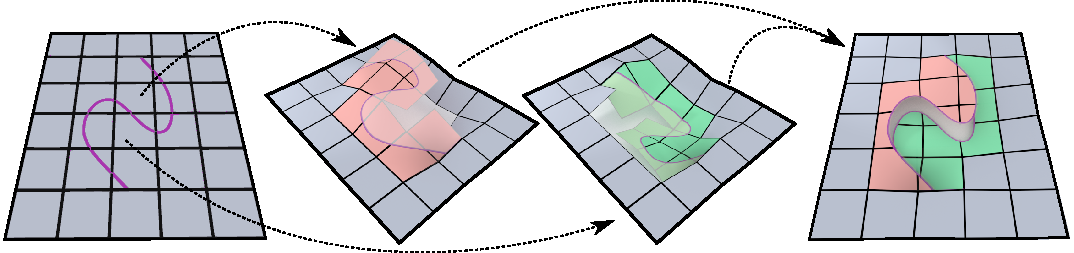
\includegraphics[width=.9\textwidth]{chapter_gridiron/images/New_HybridLattice2.pdf}
 % \includegraphics[width=.25\textwidth]{/tmp/foo.png}
\caption{Illustration of a cut generating a non-manifold lattice}{ (a) A cut
  passing through the grid. (b) Mesh cells generated for the top half
  of the cut. (c) Mesh cells generated for the bottom half of the
  cut. (d) Cut surface is colored to show cell assignment.}
\label{Fig:MaterialContinuity}
\end{figure}

We now seek to construct a coarser resolution explicit mesh
discretization, which is allowed to be non-manifold in regions, as
shown in Figure \ref{Fig:MaterialContinuity}. We will extend the
paradigm of non-manifold embedding proposed by
\citet{TeranSBNLF:2005} and 
\citet{SifakDF:2007} using the precomputed fine grid rasterization
to answer material connectivity predicates. Our non-manifold mesh
generation process is outlined in Algorithm
\ref{alg:NonmanifoldMeshGeneration}, and illustrated intuitively in
Figure \ref{Fig:MaterialContinuity}. Note that, in the pseudocode
provided, there are two geometric predicates being used: (a)
Determination of material components (line 3) requires the
identification of all disconnected components of material present in
the intersection of our domain with a given lattice cell. (b)
Adjacent-element material continuity (line 10) is a predicate invoked
to determine if two material fragments, associated with adjacent
lattice cells, exhibit material continuity across their common
face. These two geometric predicates are expressed in a fashion that
is agnostic to the underlying geometric representation of material; in
\citet{TeranSBNLF:2005} the assumption is that a
tetrahedralized model of the material is available, while \citet{SifakDF:2007} define material fragments indirectly,
by specifying cutting surfaces instead. In our case, the availability
of the fine-grid rasterization makes both such operations purely
combinatorial in nature. Material fragments within a coarse cell are
computed via flood-fill, and fragments on adjacent cells are
continuous if they contain adjacent \emph{fine} cells on their
rasterization. At the conclusion of this step, we have produced a
coarse mesh (with explicitly stored connectivity), whose topology is
as close as possible to the embedded geometry.

This generated mesh is now suitable for simulation, allowing us to
correctly embed opposite sides of a cut or thin feature in
topologically disconnected cells. However, beyond simulation, this
approach can also be valuable for detecting and handling contact
scenarios under the context of soft-body self collisions. The
remaining sections in this chapter will demonstrate how this embedding
technique can be adapted to this purpose via a technique we call
non-manifold level sets.

\section{Level Sets \& Collision Processing}
Before we discuss the details of non-manifold levelsets, it is
important to review the basic concept of a level set and how it can be
used for collision handling. Nearly three decades after their
introduction ~\citep{OsherS:1988}, level sets have evolved into one of
the most widely used representations of geometry, alongside
traditional alternatives such as meshes, splines and subdivision
surfaces. A level set implicitly represents a domain boundary
$\Gamma=\partial\Omega$ as the zero-value isosurface (i.e. zero
\emph{level set})
\begin{equation}
\Gamma=\left\{\vec{x}\in\mathbf{R}^n\ |\ \phi(\vec{x})=0\right\}
\label{eqn:definition}
\end{equation}
of a scalar field $\phi(\vec{x})$\footnote{It should be noted that the
function $\phi(\vec{x})$ used here is different than the deformation
map $\phi(\vec{X})$ described in Chapter \ref{chp:engineering},
despite the use of the same symbol.} measuring signed distances to the
boundary of the object $\Omega\subset\mathbf{R}^n$. Level sets allow
for fast $O(1)$ time point-object intersection queries or point
projections to the object surface. Model deformation is also possible,
including topological split and merge operations, simply by varying
the underlying scalar field. Level sets are used in a diverse range of
applications including surface editing ~\citep{MusetBWB:2002},
tetrahedral meshing ~\citep{LabelS:2007}, scattered point interpolation
~\citep{ZhaoOF:2001}, fluid simulation ~\citep{OsherF:2002} and collision
processing for deformable solids ~\citep{Gascu:1993}, rigid bodies
~\citep{GuendBF:2003} and skinning animations ~\citep{VaillBGCRWGP:2013}.


\begin{figure}
  \centering
\includegraphics[width=0.98\columnwidth]{chapter_nonmanifoldlevelsets/images/problem_cases.pdf}

\caption{Illustration of cases poorly handled by conventional level
  set discretizations} {Scenarios where standard Cartesian grid-based
  level sets lack the expressive ability to resolve thin features. For
  the vector art hand (top left), the cells highlighted in red show
  features that will not be resolved. While many cases can be resolved
  with fine enough resolutions, the fractured cube (bottom left) is an
  instance that cannot be resolved with conventional level sets.}
\label{fig:underresolved}
\end{figure}


% The algorithmic interface to an implicit surface data structure is
% highly dependent on the application it caters to. A fluid simulation
% application would likely mandate support for dynamic evolution of the
% interface. Geometry processing tasks may be more dependent on
% contouring or differential properties such as curvature. The data
% structure we propose, which is essentially a multivalued signed
% distance field, might require a different interface depending on the
% end application. For example, applications in multiphase
% fluids~\citep{LosasSSF:2006}, multi-material surface
% tracking~\citep{DaBG:2014} or volumetric meshing~\citep{SachtJPSS:2013}
% may contribute their own interpretations to what a non-manifold
% feature may be and what algorithmic routines need to be supported.

% The algorithmic interface of different instances of level set methods
% is highly dependent on the applications they cater to. When seeking
% unconventional extensions to the core level set formulation, it is
% important to recognize that the semantics of a \emph{multivalued or
%   non-manifold level set} can invite quite distinct interpretations in
% different use scenarios. For example, fluid simulation of multiple
% immiscible liquids \citep{LosasSSF:2006} might consider triple
% junctions as a ``non-manifold'' trait of interest, while fluid
% animations that allow different liquids to diffuse into one another
% might require modeling phase boundaries that can cross and overtake
% one another. Similarly, applications in shape modeling and collision
% processing might not concern themselves with advection tasks, but
% emphasize the signed distance property and the geometric queries it
% facilitates.

% In order to avoid such ambiguities we focus our scope to a specific
% driving application: collision detection and penalty-based response on
% volumetric simulation of elastic solids.  In section
% \ref{sec:self-collisions} we review how this specific application
% utilizes conventional (manifold) level sets, identify scenarios where
% the limitations of the traditional formulation hinder the efficacy of
% collision processing or even make it inapplicable, and explain how the
% non-manifold level set concept can alleviate those obstacles.  In
% summary, our key contributions are as follows:

% While the visual fidelity of fluid simulations is not severely
% compromised even though level sets bleed resolution, solid
% simulations run into problems when two surfaces come very close to
% each other.  This issue can arise either due to collisions or be
% inherent in the model itself (for e.g., lips, fingers and armpits in
% a human model). Interestingly, we observe that these issues are not
% intrinsic to the concept of the level set function, but rather the
% data structure that is typically used for storage.  By convention
% (or habit), standard arrays are used for storage as opposed to
% something more expressive. Normally, a level set function captures
% the (signed) distance to the surface.  By changing the underlying
% data structure, we aim to extend the definition of a level set so
% that it can capture distance to several local minima of closest
% points as well as distance to the surface along a given connectivity
% path. (Maybe refer to a figure for the lips here?)

% Self-collision in volumetric bodies gives rise to interesting
% options: a) only the surface need be processed (while elasticity
% takes care of the rest), and b) as opposed to cloth
% simulations~\citep{BarafWK:2003}, the starting state need not be
% interpenetration-free - these facts have been leveraged in
% conjunction with level sets~\citep{TeranSIF:2005,McAdaZSETTS:2011}
% even in performance-conscious environments and have proven to be
% robust in resolving extremely complex collision scenarios such as
% triple contacts. However, a significant limitation of this approach
% is that it requires the reference configuration of an object to be
% level set representable. While this is possible in some cases, it
% becomes challenging in other situations such as the lips which
% require an incredible amount of resolution to resolve the gap in
% between (note that this resolution is not required for either the
% upper lip or the lower lip in isolation, or if both lips were
% initially far apart). This problem also arises when simulating
% incisions or fracture. Similar challenges arise in applications such
% as meshing techniques that use level set representations as the
% input, in such cases an exorbitant amount of resolution might be
% required near topological features that need to be resolved in a
% voxelization of the domain.  Embedded representations suffer from
% similar problems as they have to stick to the topology of the
% embedding lattice. Our motivation comes from virtual node/XFEM
% descriptions that alleviate these issues by using a non-manifold
% mesh to capture the domain augmented with some kind of a sub-cell
% description of the domain (or its boundary). Our key idea is to use
% a fracture modeling algorithm to create a non-Euclidean embedded
% mesh structure for storing the level set function. We also show how
% peripheral operations such as reinitialization, advection and
% contouring can be extended to this new data structure.


% \begin{itemize}
% \vspace*{-.04in}\item We extend level set representations by storing
% discrete values on nodes of a non-manifold Cartesian grid, enabling
% them to represent domains with thin gaps or slivers, and even encode
% boundaries of overlapping material domains.

% \vspace*{-.08in}\item We detail a systematic pipeline for converting
% mesh-based geometry representations into multivalued level sets, and
% discuss how other geometric descriptions
% % (e.g. fracture boundaries)
% could also be used as input.

% \vspace*{-.08in}\item We extend a number of algorithmic concepts and
% geometric predicates, such as signed distance initialization and
% closest-point projection to the non-manifold level set paradigm.

% \vspace*{-.08in}\item We show how non-manifold level sets can
% broaden the scope of penalty-based self-collision processing for
% elastic solids.

% \end{itemize}
% \vspace*{-.1in}

% \section{Previous work}
% \vspace*{-.1in}
% \label{sec:previous-work}

% Level set methods were first introduced \changed{by Osher and
%   Sethian~\citet{OsherS:1988}}{in~\citep{OsherS:1988}} for tracking
% moving interfaces in the context of Hamilton-Jacobi equations.
% Subsequently, \changed{Adalsteinsson and
%   Sethian~\citet{AdalsS:1994}}{\citep{AdalsS:1994}} proposed
% substantial \changed{runtime savings }{savings to the run-time }by
% restricting computations to a thin band of active voxels near the
% interface.
% \changed{Sethian~\citet{Sethi:1998}}{\citep{Sethi:1998}} proposed
% fast marching methods for monotonically advancing fronts as well as
% for redistancing the level set using values seeded only on the narrow
% band.  Besides fast computation, a number of methods have also been
% proposed for efficiently storing level sets including
% octrees~\citep{LosasGF:2004}, RLE
% representations~\citep{HoustNBNM:2006,IrvinGLF:2006,ChentM:2011}, the
% VDB data structure~\citep{Muset:2013} which evolved from Dynamic
% Tubular Grids~\citep{NielsM:2006} and the DB+Grid data
% structure~\citep{Muset:2011}, and the virtual-memory based SPGrid data
% structure~\citep{SetalABS:2014}.

% Methods have been proposed for computing implicit representations of
% non-manifold surfaces~\citep{BloomF:1995,YuanYW:2012}. Similar ideas
% were used for simulating bubbles~\citep{ZhengYP:2006} and multiphase
% fluids~\citep{LosasSSF:2006}. Our work diverges from these approaches
% as we enhance the expressive capability of a \emph{single} level set
% by embedding signed distance values on an explicit mesh. Our work is
% related to the practice of embedding high-resolution geometry in
% regular meshes, a concept that was first leveraged \changed{by
%   M\"{u}ller et al.~\citet{MulleTG:2004}}{in~\citep{MulleTG:2004}}
% for deformable body simulations and fracture.  In addition to
% hexahedral embeddings, methods such as the virtual node
% algorithm~\citep{MolinBF:2004} have been used to create non-manifold
% tetrahedral lattices that correspond to thin topological features in
% the embedding geometry. Virtual node concepts are also similar to XFEM
% methods which were used for crack modeling~\citep{MoeesDB:1999} and for
% cutting and fracturing thin shells~\citep{KaufmMBGG:2009}. This
% principle has continued to evolve with many of the topological
% limitations in prior approaches being raised \changed{by Sifakis et
%   al.~\citet{SifakDF:2007}}{in~\citep{SifakDF:2007}} and has been
% successfully used in production tools as well~\citep{HellrSSST:2009}.

% Our non-manifold level set approach is inspired by these methods, but
% it needs to be made cognizant of further topological limitations that
% the signed distance field imposes on our representation (see
% Section~\ref{sec:non-manifold-level-sets}). Notably, when dealing with
% collisions near thin features, all of the aforementioned approaches
% employed detection and response techniques based on surface
% meshes~\citep{BridsFA:2002} that rely on the availability of good
% surface meshes, are computationally expensive, presume collision-free
% history or use impulses which makes implicit integration
% challenging. To accelerate collision detection and response while
% allowing for implicit integration, methods have been proposed using
% implicit surface representations~\citep{McAdaZSETTS:2011} which work
% even in near-interactive settings, but require enough level set
% resolution to avoid any non-manifold features altogether. Recently,
% image-based techniques~\citep{FaureBAF:2008,WangFP:2012} have been
% proposed which provide an interesting alternative.  Finally, implicit
% surfaces have also been recently used in real-time skinning
% applications~\citep{VaillBGCRWGP:2013,VaillGBWC:2014}.

\subsection{Level set collisions for volumetric solids}
\label{sec:self-collisions}

% We present our new implicit surface formulation in the context of
% collision processing for elastic volumetric bodies.

Self-collision processing is paramount in generating visually attractive and
realistic shapes, as is evident in character skinning pipelines
~\citep{McAdaZSETTS:2011,VaillBGCRWGP:2013}. Handling collisions in
volumetric solids can be quite different than the typical cloth
collision pipeline. With volumetric solids there is a clear
distinction between an \emph{inside} and an \emph{outside} region,
making it possible to process collisions in a single time instance of
a simulated deformation. In contrast, if collisions are detected in a
cloth simulation, we need to rely on deformation history to determine
how the cloth surface is to be untangled (unless global intersection
analysis~\citep{BarafWK:2003} is performed). While cloth simulations
typically strive for a collision-free state at all times, commonly
enforced via impulses in semi-implicit integration
schemes~\citep{BridsMF:2003}, volumetric objects can tolerate
occasional, limited interpenetration, and respond to collision with
penalty forces which are more easily coupled with explicit integration
schemes. In this section, we review a level-set assisted technique
that capitalizes on these opportunities to handle volumetric object
collisions in large time-step implicit integration schemes, without
requiring a collision-free deformation history.  In section
\ref{sec:non-manifold-level-sets} we explain when standard level sets
are inadequate for this task, and use this as motivation for our
non-manifold variant.

\begin{figure}
  \centering
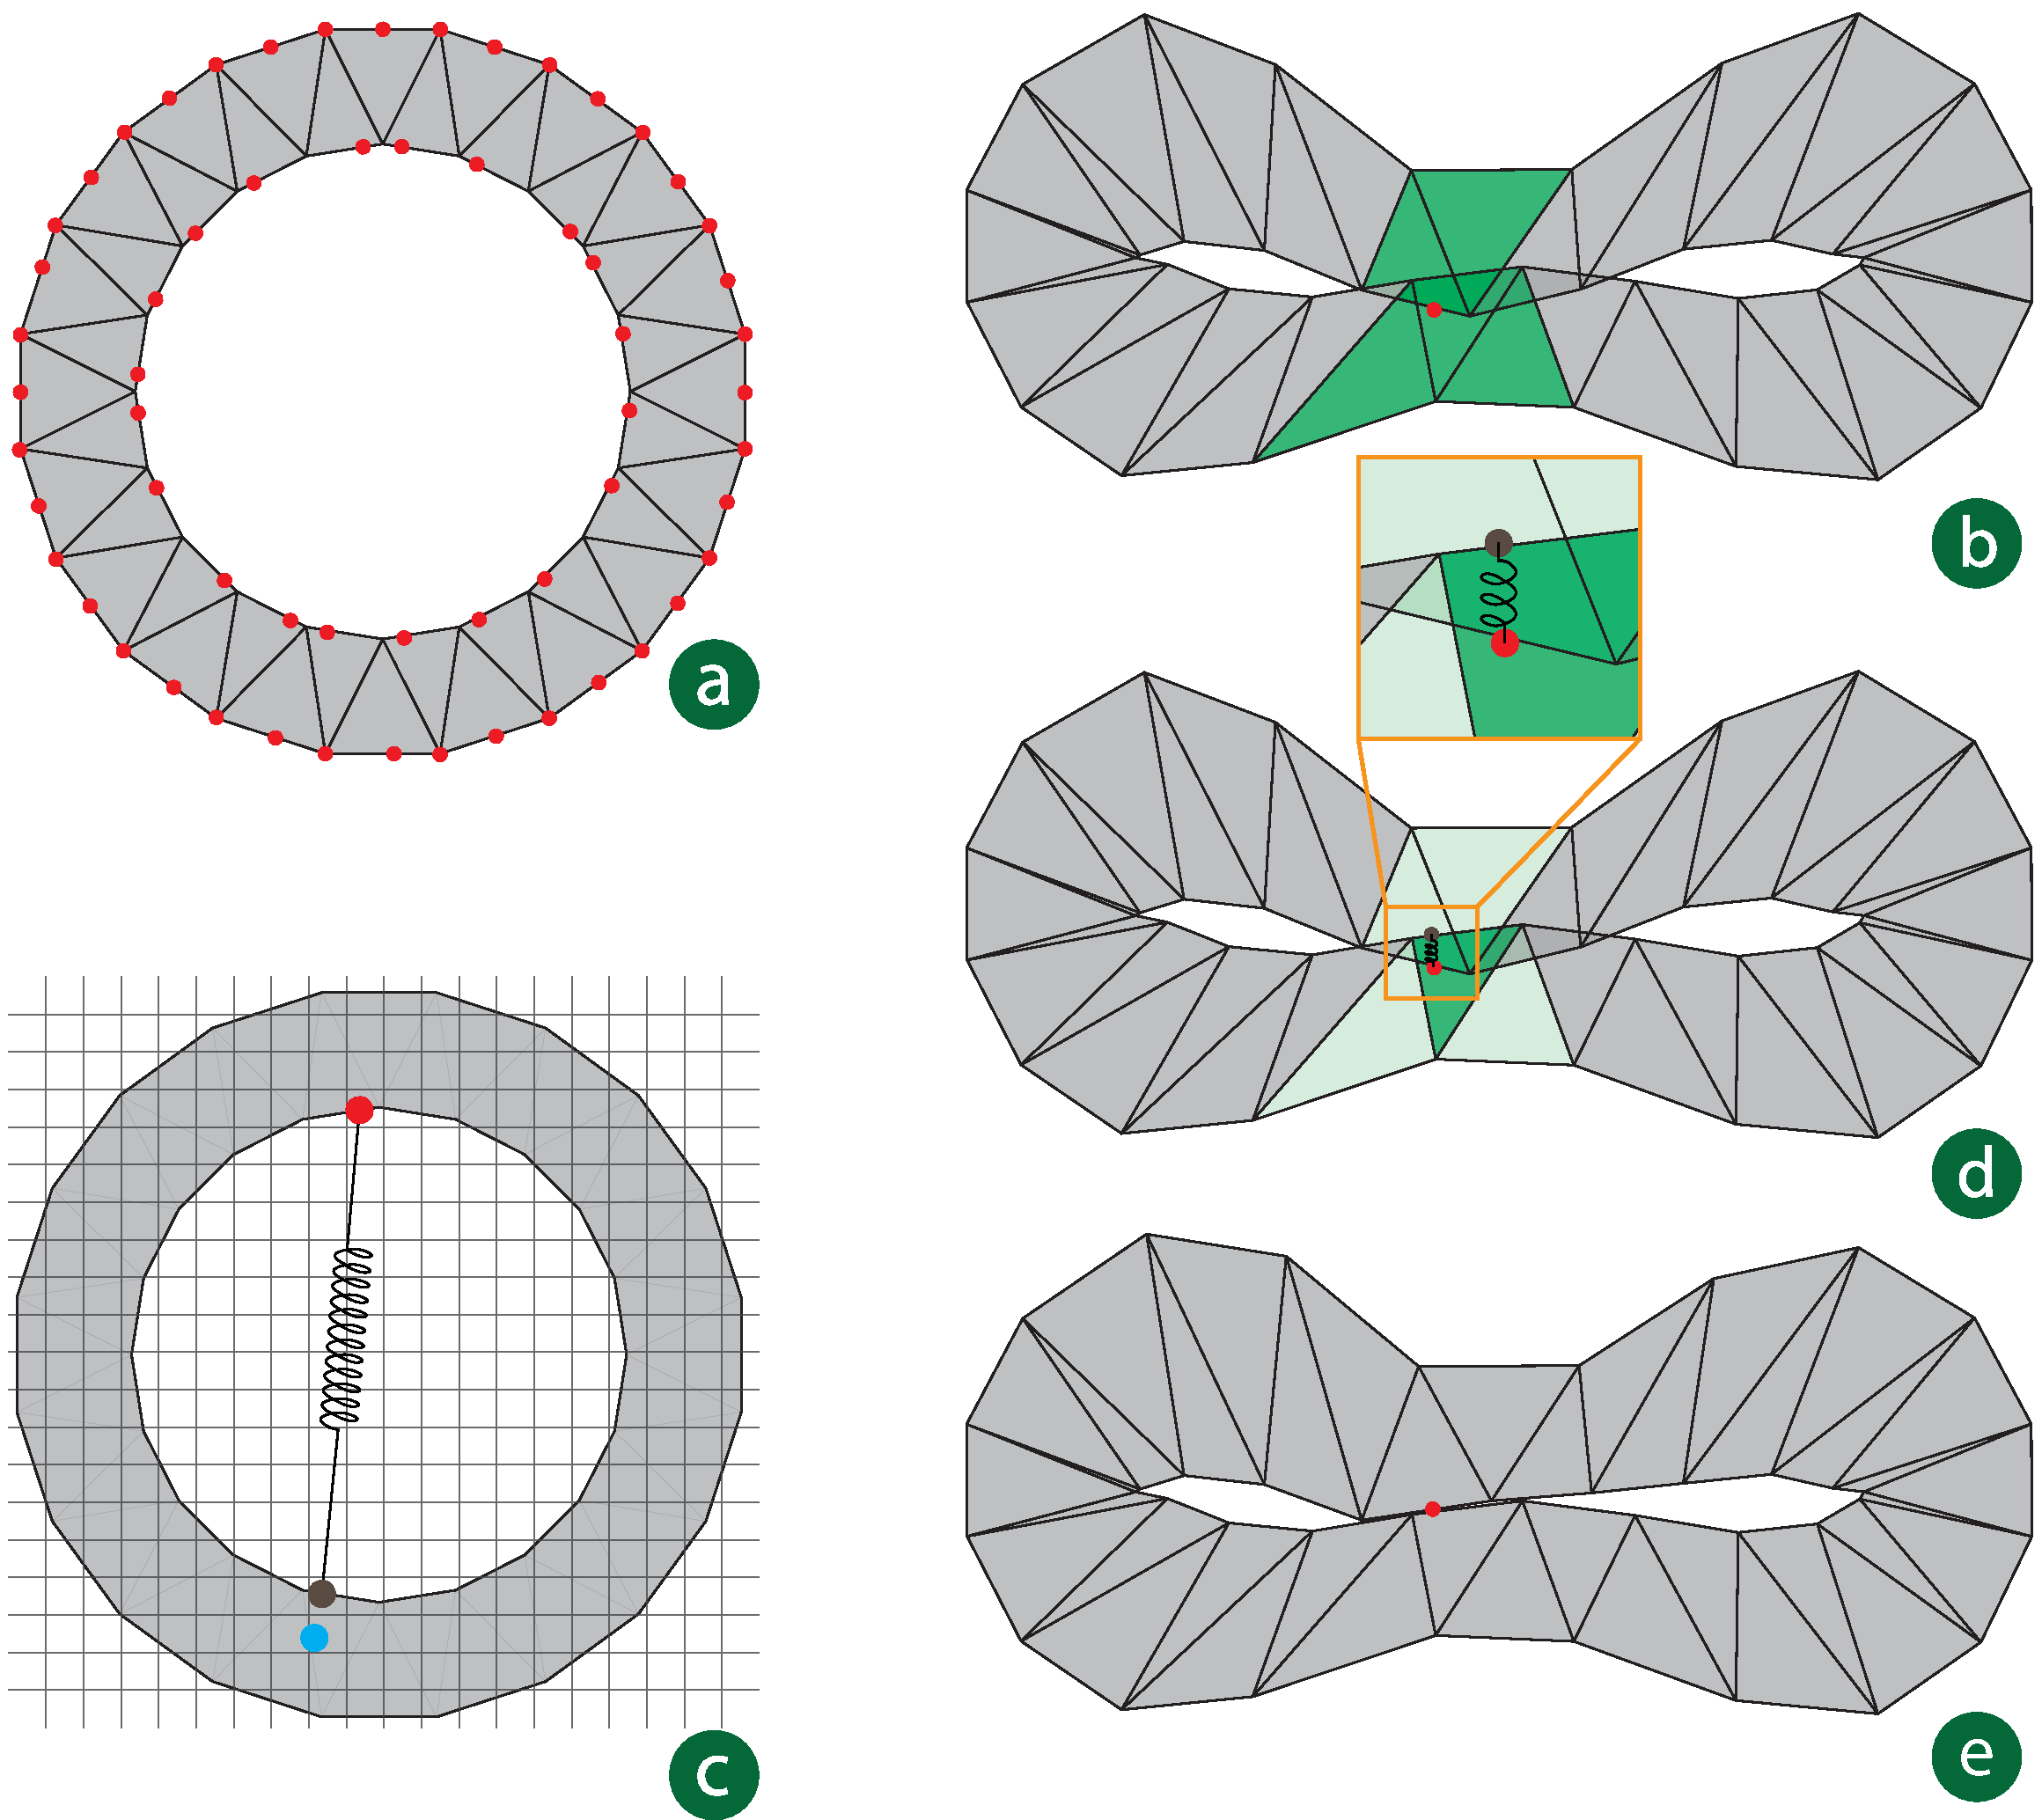
\includegraphics[width=0.95\columnwidth]{chapter_nonmanifoldlevelsets/images/torus-combined-latest.pdf}
\caption{Illustration of the self-collision pipeline}{(a) a
  triangulated torus model is pictured in its undeformed
  configuration. Collision proxies on the surface shown in red.  (b)
  The torus is deformed into a self-colliding state. A bounding box
  hierarchy yields initial candidates of triangles colliding with the
  proxy.  (c) After pruning false positives, the material location
  that the proxy collided onto is identified, and mapped back to the
  undeformed configuration (blue dot). The level set (stored on the
  pictured grid) is used to project to the closest surface point
  (brown dot).  (d) A zero-rest spring is initialized between the
  proxy and its surface-projected target.  (e) The deformed torus
  after the self-collision is resolved.}
\label{fig:self-collision-handling}
\end{figure}


Our collision pipeline consists of two stages: In the detection stage,
discrete material points (labeled \emph{collision proxies}) are
checked for collision against the object interior. In the response
stage, we use a spring-like penalty force to push each colliding proxy
to the object surface~\citep{TeranSIF:2005,McAdaZSETTS:2011}. Since
simulated solids are typically endowed with elastic material models
that prevent (or discourage) inversion, in all our examples we chose
to only seed collision proxies on the object surface, as internal
non-inversion combined with boundary non-collision would imply a
globally non-intersecting state. Interior collision proxies can also
be used, if desired, with no algorithmic
change. Figure~\ref{fig:self-collision-handling} illustrates the
detection and response process on an elastic torus model squished into
self-collision. For any colliding proxy, we identify the offending
(internal) material location that the proxy collided with. The closest
surface point to that material location is calculated, and a zero
rest-length spring is introduced between that surface location and the
original proxy. This spring remains active just until the collision
detection phase is repeated; typically for one step of the time
integration method employed, or for just a single Newton iteration in
an implicit scheme. The most costly predicates in this process are (i)
detecting whether a proxy intersects the object interior, and (ii)
projecting the offending location to the model surface. Both
predicates could be answered in $O(1)$ if a level set representation
of the model was available; unfortunately, the continuous deformation
makes updating an implicit representation impractical. Hence, we opt
for an \emph{approximate} algorithm ~\citep{McAdaZSETTS:2011} that only
relies on a level set representation of the \emph{undeformed} model.

For simplicity, let us assume that the deformable volumetric solids
are tetrahedralized (we can make this choice without loss of
generality - the following algorithm applies equally well to
hexahedral discretizations). Let $E_i$ denote the $i$-th simulation
element in the undeformed configuration and $e_i$ denote the same
element in the deformed configuration. Similarly, let $P_i$ denote the
location of the $i$-th collision proxy in the undeformed configuration
and $p_i$ denote its deformed counterpart.  Collision proxies can be
regularly sampled on the \emph{surface} of the simulated object, or
the surface vertices of the embedded object themselves can be used as
proxies, if their distribution is reasonably regular\footnote{Proxy
  spacing is an important task, though somewhat tangential to
  this conversation. Too few proxies in a region can lead to poor
  collision response or excessive penetration. Too many proxies can
  lead to an over-constrained problem, resulting in slow convergence or
  other unfortunate artifacts. For our system, a Poisson-disk
  sampling technique ~\citep{CorsiCS:2012,Devro:1986} was used to generate a blue noise pattern
of proxies over the model surfaces.}.  Let $\phi$
denote the level set function for the simulated volume in the
undeformed configuration. The collision handling routine performs the
following steps for each proxy $p_i$\ :

\textbf{Step 1}\ \ The set of (deformed) elements $\mathcal
  E=\{e_{i_1},e_{i_2},\ldots,e_{i_k}\}$ are checked against $p_i$ for intersection. This is performed as follows:

  \begin{enumerate}[(a)]
    \item We use an axis-aligned bounding box
    hierarchy, defined over all deformed elements, to identify all
    elements whose bounding box intersects $p_i$, i.e.\
    $\mathcal{E}_{\mbox{\small
        int}}=\{e_k\in\mathcal{E}|\texttt{Box(}e_k\texttt{)}\cap
    p_i\neq\emptyset\}$.

    \item We identify the element $E_i$ that contains the proxy
    $P_i$ in the undeformed configuration. This may be more than one element,
    e.g.\ if $P_i$ was a mesh vertex. We trivially have that
    $e_i\in\mathcal{E}_{\mbox{\small int}}$, as $p_i$ is embedded in it.
    Similar to \citet{McAdaZSETTS:2011}, we prune $e_i$ along with all of its immediate topological neighbors from
    $\mathcal{E}_{\mbox{\small int}}$, since collision response between
    primitives that share embedding parents can be problematic
    (instead, we rely on
    elasticity to discourage extreme cases of local collision).

% Element $e_i$ and its topological neighbors
%    are discarded from the computed set, where $P_i$ is embedded
%    inside $E_i$ in the rest configuration. This is done to prune
%    false negatives, as the proxy will trivially intersect its own
%    topological neighborhood.

    \item We perform an exact intersection test
    between any elements $e_t$ that have not been already pruned. We
    do so by computing the barycentric coordinates of $p_i$ with
    respect to $e_t$, and discard elements if those coordinates are
    out of bounds.

  \end{enumerate}
   \textbf{Step 2}\ \ For every colliding proxy, we
  identify the location $X_t$ in the \emph{undeformed} configuration
  of the material point the proxy impacted\footnote{Note that the location $X_t$ is unique if the element
$E_t$ is a triangle in two spatial dimensions or a tetrahedron in
three spatial dimensions, but this may not be the case for polygonal
or polyhedral elements such as squares, hexahedra, etc. We first
triangulate or tetrahedralize such elements, which can result in
several locations $\{X_{t_1},X_{t_2},\ldots,X_{t_r}\}$ in the rest
configuration corresponding to each of these several
triangles/tetrahedrons. In this case, we initialize the spring between
$p_i$ and the point $y_{t_j}$, where $X_{t_j}$ is \emph{closest} to
the surface.}. We do so using the
  barycentric coordinates computed in step 1(c) to interpolate $X_t$
  from the \emph{undeformed} colliding element $E_t$.
  \\
  \textbf{Step 3}\ \ Elements $E_t$ with $\phi(X_t)\!\!>\!\!0$ are
  dismissed as non-colliding (this could be due to discretization
  discrepancy between mesh and level set, or if an embedded simulation
  approach is used where elements in $\mathcal{E}$ reach beyond the
  extent of the simulated model).
  \\
  \textbf{Step 4}\ \ Using the level set, point $X_t$ is projected to
  the surface point $Y_t=X_t\!-\!\phi(X_t)\nabla\phi(X_t)$, for all
  elements $E_t$, where $e_t\in\mathcal{E}_{\mbox{\small int}}$.
  \\
  \textbf{Step 5}\ \ In the deformed configuration, a zero rest-length
  spring is initialized between points $p_i$ and $y_t$ to resolve the
  collision.

%\vspace*{-.2in}
  In step 5, $y_t$ corresponds to the point $Y_t$ in the deformed
  configuration.  Note that our algorithm, in steps 3 and 4, relied
  upon a level set representation of the \emph{undeformed} shape of
  the simulated model. The cost paid for this convenience is that the
  surface location $y_t$ (the collision target) is only an approximate
  surface projection in the \emph{deformed} configuration;
  nevertheless, this disparity vanishes as the effect of the collision
  springs progressively brings the penetration depth closer to zero.

Figure~\ref{fig:self-collision-handling} illustrates the
individual steps of the algorithm on a torus in two spatial
dimensions.


\section{Non-manifold Level Sets}
\label{sec:non-manifold-level-sets}

In principle, based on equation (\ref{eqn:definition}) a level set
could represent any object $\Omega\subset\mathbf{R}^n$. In practice,
however, the scalar field $\phi(\vec{x})$ is never provided
analytically, but  instead sampled at discrete points in
$\mathbf{R}^n$. As a consequence, the expressive ability of discrete
level sets is limited by the sampling resolution and the interpolation
scheme used. In the common practice where $\phi$ values are sampled on
the nodes of a uniform Cartesian grid, and trilinear interpolation is
used to define a continuous scalar field, models with multiple
boundary crossings per grid edge (near narrow gaps or strips, see
Figure~\ref{fig:underresolved}) cannot be represented. These issues
can be alleviated to some extent by using adaptive schemes
~\citep{LosasGF:2004,Muset:2013} to concentrate resolution near fine
features, or hybridizing with point-based methods ~\citep{EnrigMF:2002}
to capture details at a sub-cell level. Nevertheless, gratuitously
increasing the level set sampling resolution is a brute-force remedy
which quickly becomes impractical if the thickness of topological gaps
approaches zero, as is commonly the case with geometries arising from
cutting and fracture modeling pipelines (see
Figure~\ref{fig:zplasty-and-net}(top)). It is also unfortunate that
even though level sets are perfectly capable of localizing the
implicit surface to sub-cell resolution (trilinearly interpolated
level sets on Cartesian grids converge quadratically to surfaces of
bounded curvature) they cannot resolve multiple interface crossings
within a single cell.

Furthermore, the self-collision algorithm outlined in
Section~\ref{sec:self-collisions} works well only when a good quality
level set can be computed from the model's undeformed
configuration. In such cases, it provides the opportunity for
excellent performance, even allowing interactive simulation for highly
detailed models ~\citep{McAdaZSETTS:2011}, as it allows very aggressive
integration time steps (tolerating occasional mild inter-penetration)
and exploits the fast intersection/projection level set queries. The
approach breaks down, however, in cases where the object cannot be
resolved by the level set resolution. As a brute-force remedy, it might be
possible to pose a model in a \emph{reference configuration} that
avoids thin features (e.g. modeling a hand such that the fingers are
generously separated ~\citep{McAdaZSETTS:2011}). However, this
pre-processing can be tedious (e.g. for faces with narrow clearance
between the lips), unnatural (if the ``reference pose'' is not really
a \emph{rest} pose, see the elastic coil in
Figure~\ref{fig:underresolved}), or impossible to perform a priori if
the thin features arise during simulation (e.g. cracks and cuts). We
propose a principled remedy, designing a new implicit geometry data
structure that fully supports the necessary geometric predicates, but
accommodates models with narrow gaps or even material overlap.

We argue that these apparent limitations of level sets are not
intrinsic defects of the implicit representation (equation
\ref{eqn:definition}), but consequences of the data structure (e.g.\
Cartesian grid) conventionally used to store the signed distance
values. Instead of using $\mathbf{R}^n$ as the domain of
$\phi(\vec{x})$, we propose to define this scalar field over an
explicit quadrilateral (2D) or hexahedral (3D) mesh. We use regular
(square or cube) elements in these meshes, identical in shape to the
cells of a conventional Cartesian grid. However, the explicit
connectivity in our mesh allows us to have multiple overlapping
elements associated with geodesically distant regions (see Figure
\ref{fig:non-manifold-level-set-generation}). Furthermore, this
enables us to introduce non-manifold connectivity to capture
topological bifurcation at the tip of a crack or incision, or in the
vicinity of highly concave regions (see Figure
\ref{fig:transition-face}).

\subsection{Review: Basic non-manifold embedding}
\label{sec:stockembedding}

\begin{figure}
\centering
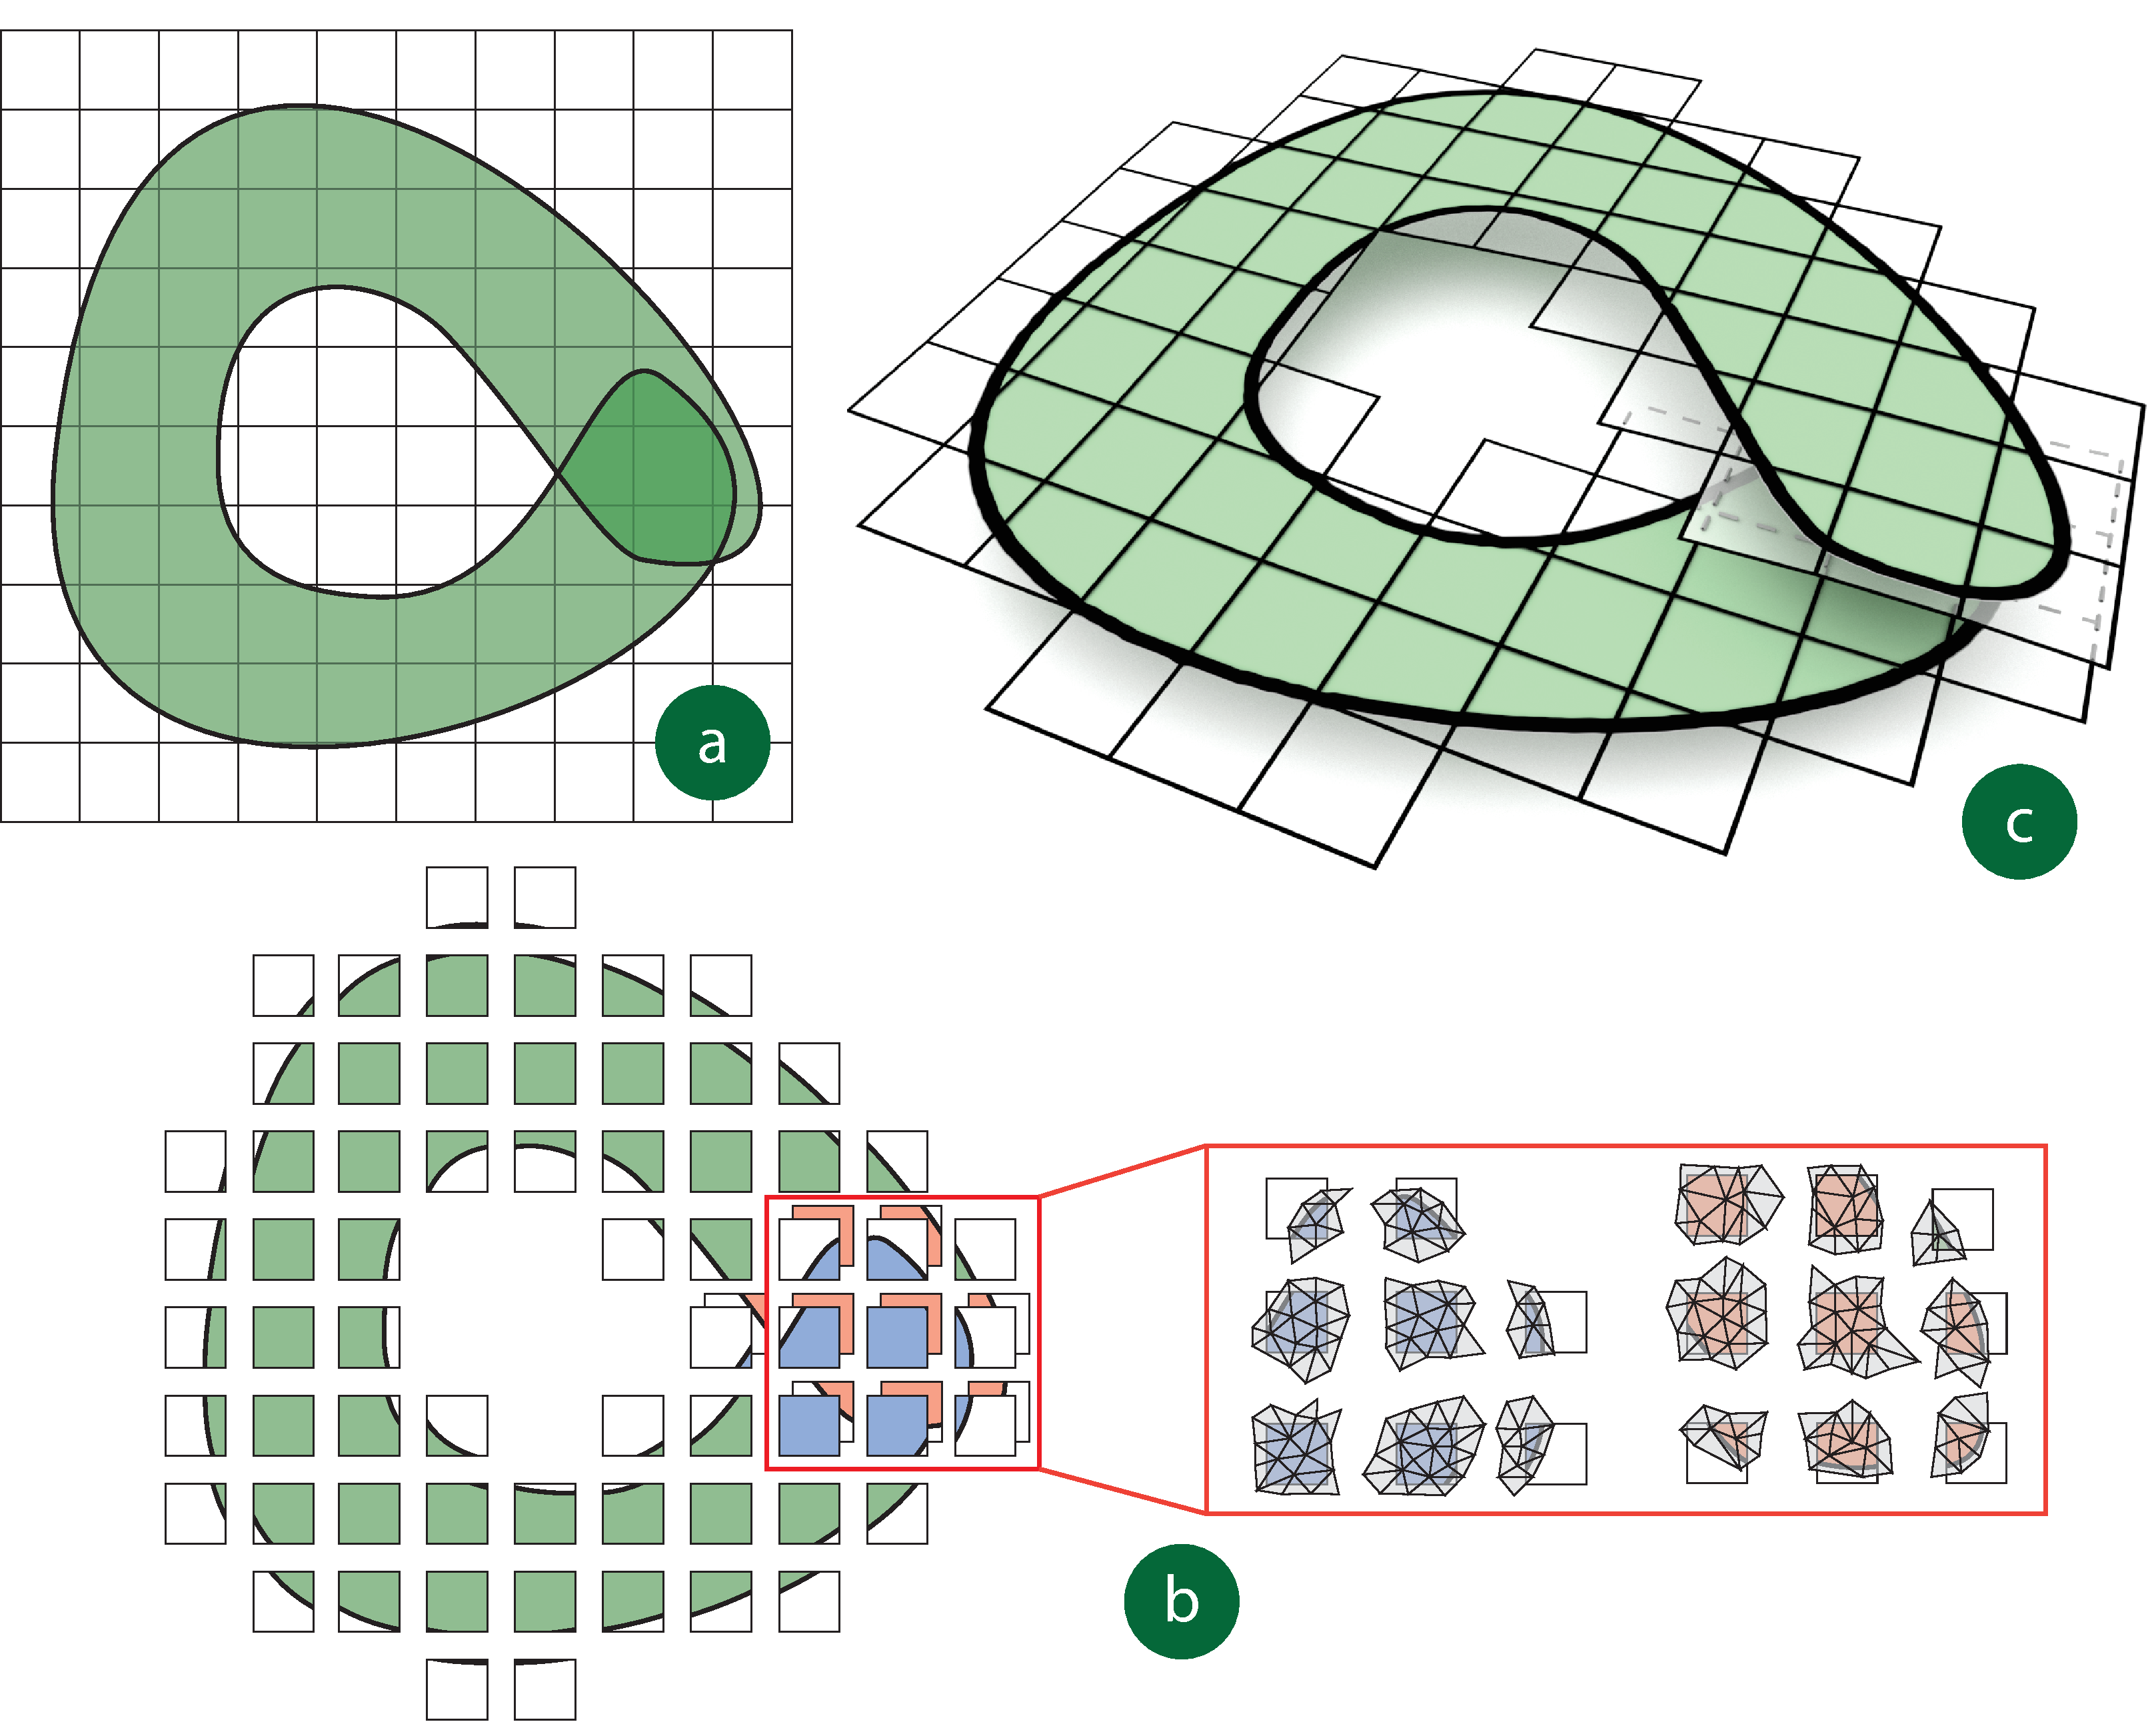
\includegraphics[width=.91\columnwidth]{chapter_nonmanifoldlevelsets/images/cshape_strip2.pdf}
\caption{Illustration of non-manifold mesh construction}{(a) A
  self-overlapping 2D model with template mesh overlaid. (b) Duplicate
  elements created during non-manifold embedded mesh generation, along
  with their associated material fragments. (c) Final non-manifold
  embedding mesh.  }
\label{fig:non-manifold-level-set-generation}
\end{figure}

Models such as the ones illustrated in Figure~\ref{fig:underresolved}
have been known to pose challenges not just for level set generation,
but also for certain dynamic simulation techniques even in the absence
of collision processing. Of course, simulation of elastic deformation
is a straightforward proposition, e.g.\ using the Finite Element
Method~\citep{SifakB:2012}, if an explicit tetrahedral mesh
representation of the model is available. However, if we wish to use
lattice deformer techniques, capable of high degrees of performance
optimization~\citep{RiverJ:2007,McAdaZSETTS:2011,MitchCS:2015}, we run
the risk of ``tying'' together disconnected material regions if they
are separated by a distance smaller than the embedding mesh resolution
(e.g.\ adjacent helices of the coil, or the two lips of the face model
pictured in Figure~\ref{fig:underresolved}). Fortunately, as we saw
earlier in this chapter, we have algorithms designed for constructing
embedding lattices capable of handling these thin incisions and fine
features. These methods add non-manifold connectivity to the embedding
mesh, duplicating elements and degrees of freedom as necessary to best
capture the embedded model topology.


Before discussing the details behind our non-manifold level sets, we
will take a moment to review a common formalism of the non-manifold
embedding process ~\citep{SifakDF:2007}. The algorithm is illustrated in
Figure~\ref{fig:non-manifold-level-set-generation}. This algorithm is
very similar to the one presented in Algorthim
\ref{alg:NonmanifoldMeshGeneration}, except here we are assuming a
material predicate defined by a triangulation (or tetrahedralization
in 3D). We do this partially to show how the algorithm adapts to
multiple material description predicates, but also to support models
with zero width cuts and overlapping geometry. These later aspects are
not supported by the discrete fine grid as presented earlier in the
chapter. The choice of material description is somewhat arbitrary - a
decision made around what geometric features one needs to capture. 

\textbf{Input:} (a) A geometric description of the shape to be
embedded (the green-shaded area in
Figure~\ref{fig:non-manifold-level-set-generation}). For simplicity,
we may assume the geometry is given as a triangulated model, which
allows us to express the self-overlap in our specific example. (b) A
mesh which will be used as a \emph{template} for our embedding
process. In Figure~\ref{fig:non-manifold-level-set-generation}(a) this
is the regular quadrilateral mesh pictured in the foreground.
\\
\textbf{Step 1 [Element separation]} We separate each element of the
template (quadrilateral) mesh, keeping track of the subset of our
material model that is contained in each such element (e.g.\ taking
note of all material triangles that intersected each quadrilateral).
\\
\textbf{Step 2 [Element duplication for disconnected components]} For
each embedding element, we identify all disjoint connected components
of material contained therein (e.g.\ by checking connectivity of the
respective material triangles). We generate a \emph{duplicate}
embedding (quadrilateral) element for each material component. Note
that, at this point, all embedding elements are still disconnected.
\\
\textbf{Step 3 [Restoring connectivity]} For any pair of
\emph{geometrically} adjacent embedding elements, we check if there is
material continuity across their common face (e.g.\ by checking if
they both intersect the same material triangle on that face). If such
continuity exists, we collapse all vertices along their common
face. This collapse is transitive; in the example of
Figure~\ref{fig:transition-face}(left) all three elements near a
convex material region have acquired a common face (with non-manifold
connectivity) due to transitive pair-wise vertex collapses.

The result is shown in Figure~\ref{fig:non-manifold-level-set-generation}(c); after discarding embedding elements with no material content, the final embedding
mesh has been fully assembled, with overlapping duplicates of elements properly connected, respecting the topology of the embedded material.

 
\subsection{Mesh bifurcation and transition faces}

\begin{figure}
  \centering
  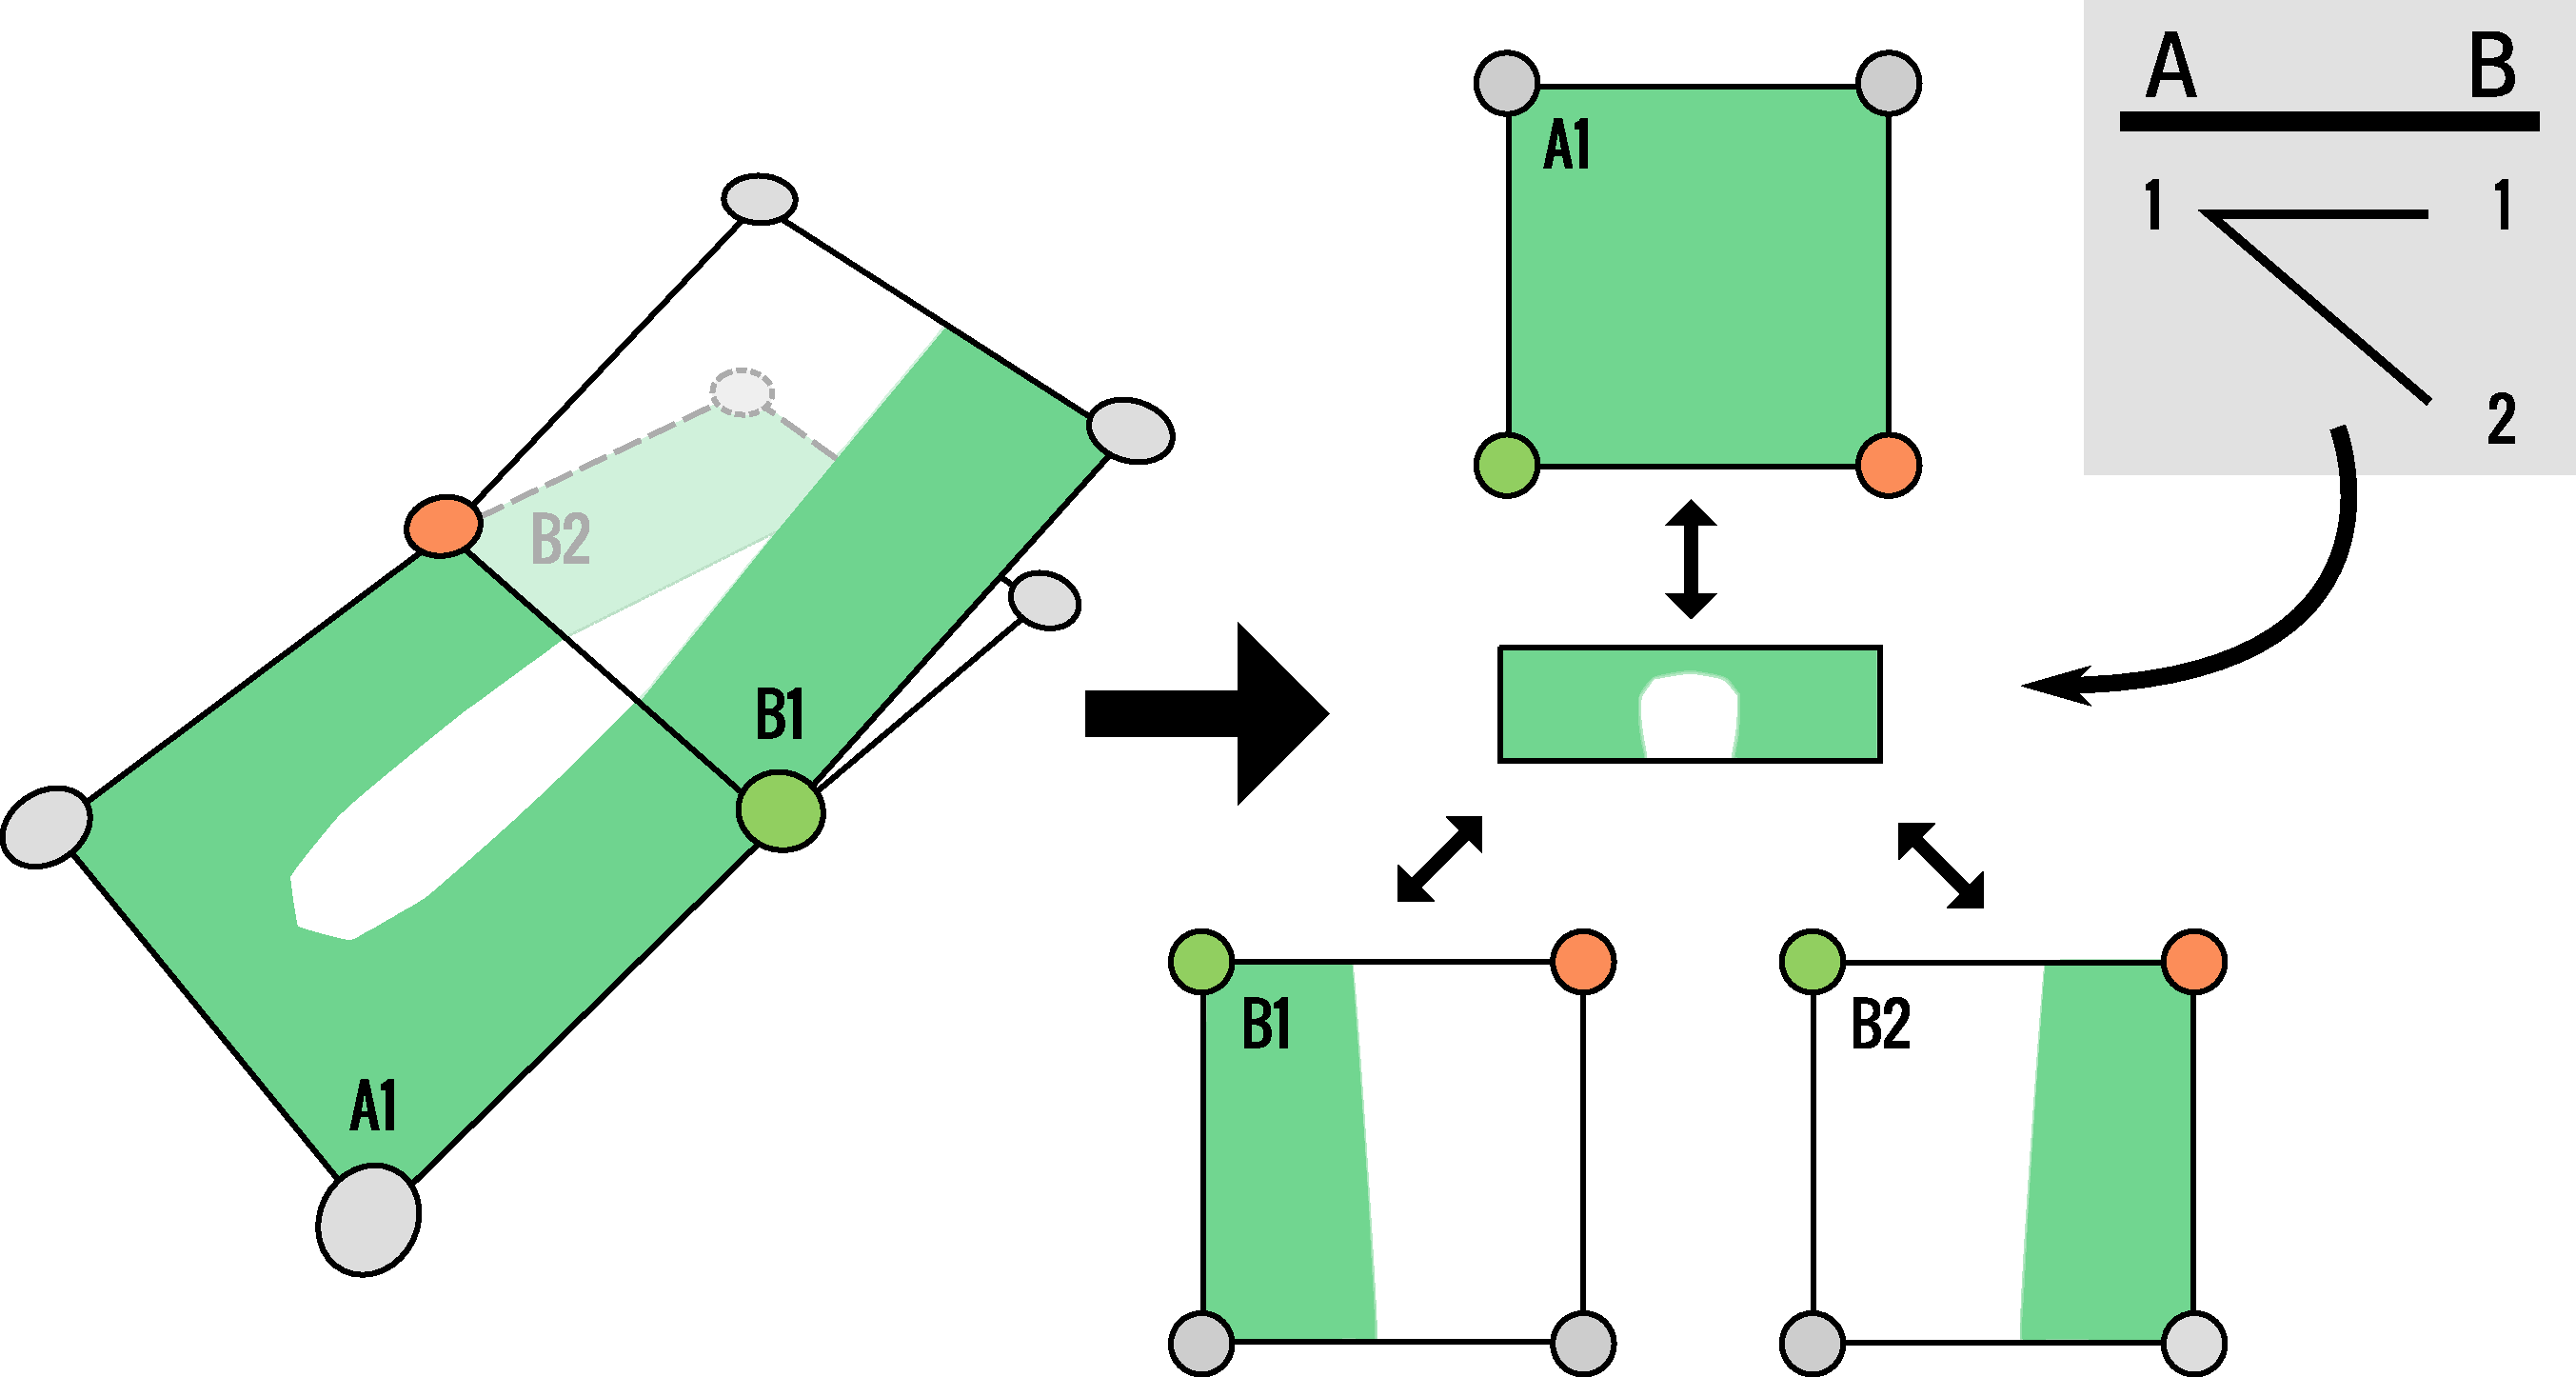
\includegraphics[width=.8\columnwidth]{chapter_nonmanifoldlevelsets/images/TransitionFaceNew2.pdf}
  \caption{Illustration of handling material bifurcations}{(Left) An example where material bifurcates at an edge in a
    non-manifold Cartesian embedding. (Right) Level sets can only
    store a single interface transition at an edge. In the
    non-manifold level set bifurcations are explicitly recorded in
    \emph{transition faces} that record a connectivity graph between all cells on
    the left and right.}
  \label{fig:transition-face}
\end{figure}

The intent of our proposed level set data structure would be to store
signed distance values on the \emph{nodes} of the embedding mesh
produced by the algorithm just described (to our knowledge, these
\emph{non-manifold} embedding meshes have only been previously used to
store deformation data, not level set values). Of course, such signed
distances would be computed geodesically, along the embedding mesh,
rather than in the Euclidean sense. Subsequently, a continuous signed
distance field would be computed on the embedding mesh via standard
bilinear (2D) or trilinear (3D) interpolation. We note that in
``simple'' cases such as the example of
Figure~\ref{fig:non-manifold-level-set-generation} (where we have
element overlap, but no non-manifold connectivity) this approach would
have been fully sufficient. Unfortunately, scenarios such as the one
illustrated in Figure~\ref{fig:transition-face}(left) reveal a
newfound challenge: elements hinged in a non-manifold configuration on
a common face may disagree on the \emph{sign} of the signed distance
value stored on one of their common vertices. In
Figure~\ref{fig:transition-face}(left), elements \textsf{A1} and
\textsf{B2} record the vertex in orange as being inside the material
domain (hence carrying a negative level set value), while the same
vertex is outside the embedded domain (with a positive level set
value) as far as element \textsf{B1} is concerned. At this point, we
should emphasize that any discrete level set is an inherently
approximate representation of geometry, as it depends on interpolation
of signed distance value samples. The severity of this phenomenon,
however, is much greater as it carries the risk of eliminating parts
of the model boundary, or forcing it to spuriously appear in parts of
the embedding mesh that it did not originally traverse.  Note that
this behavior does not affect non-manifold embedding for simulation
purposes, since such techniques explicitly track the material embedded
in each element, rather than using interpolated vertices. 

\begin{figure}
  \centering
\subfloat{
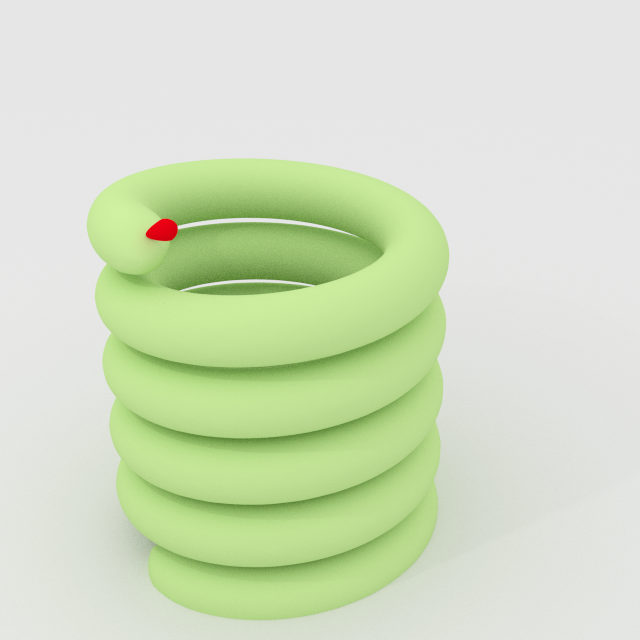
\includegraphics[height=.2\paperheight]{chapter_nonmanifoldlevelsets/images/coil_001.png}
\hfill
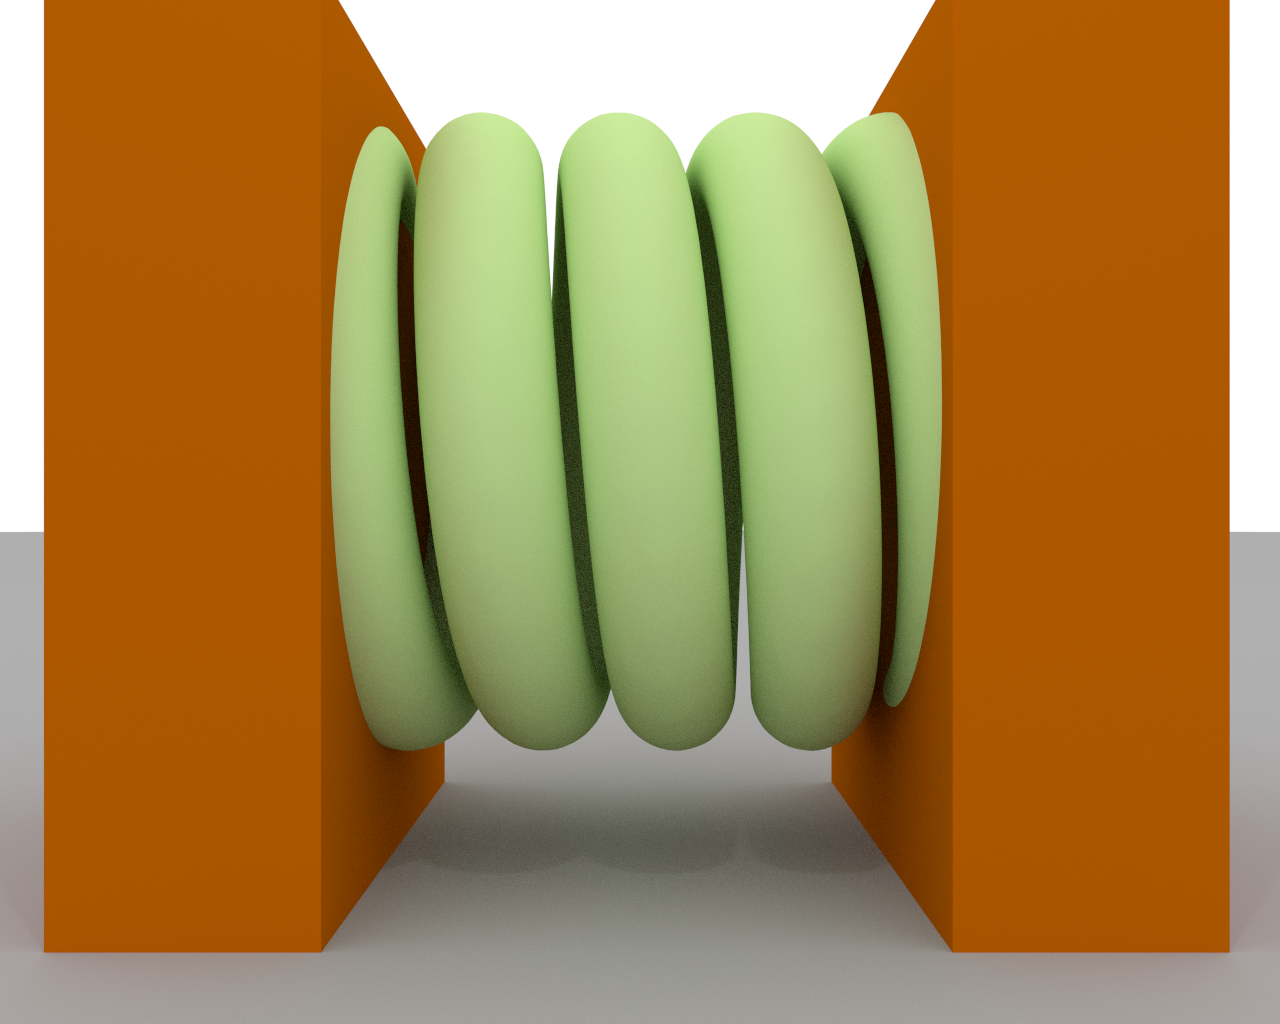
\includegraphics[height=.2\paperheight]{chapter_nonmanifoldlevelsets/images/compression_001.png}
}
\subfloat{
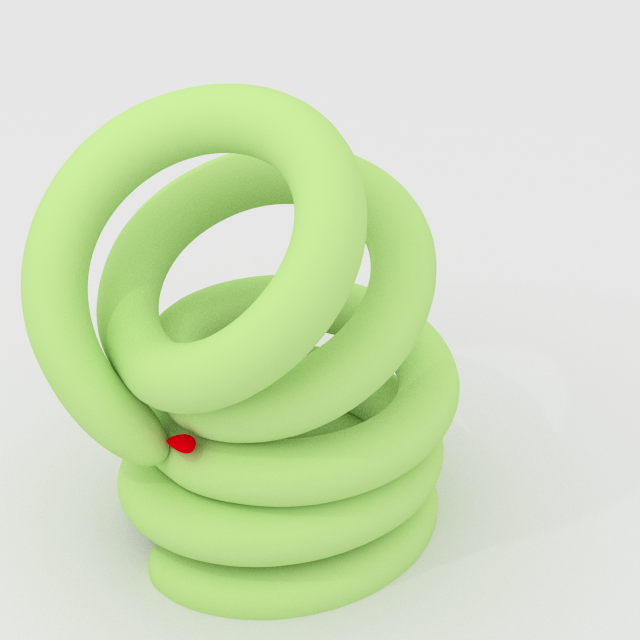
\includegraphics[height=.2\paperheight]{chapter_nonmanifoldlevelsets/images/coil_040.png}
\hfill
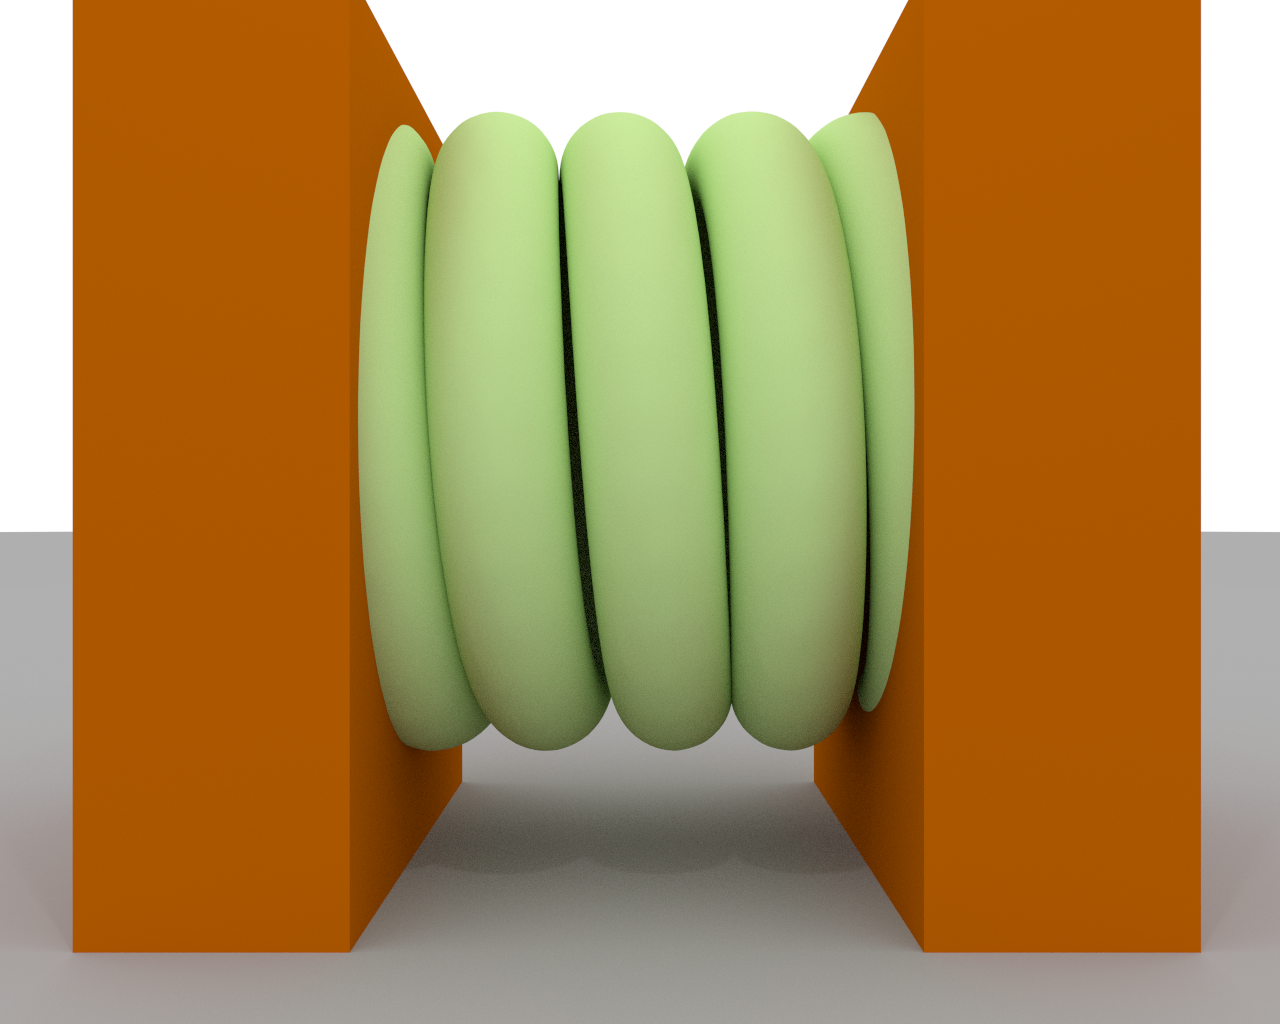
\includegraphics[height=.2\paperheight]{chapter_nonmanifoldlevelsets/images/compression_005.png}
}
\subfloat{
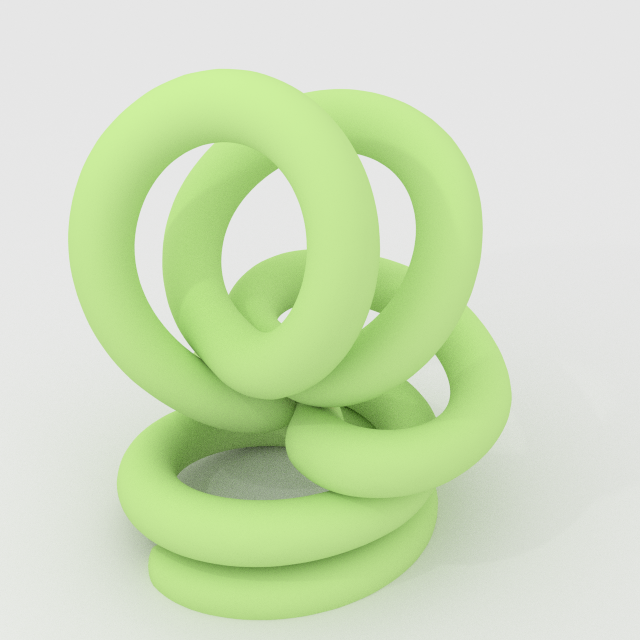
\includegraphics[height=.2\paperheight]{chapter_nonmanifoldlevelsets/images/coil_065.png}
\hfill
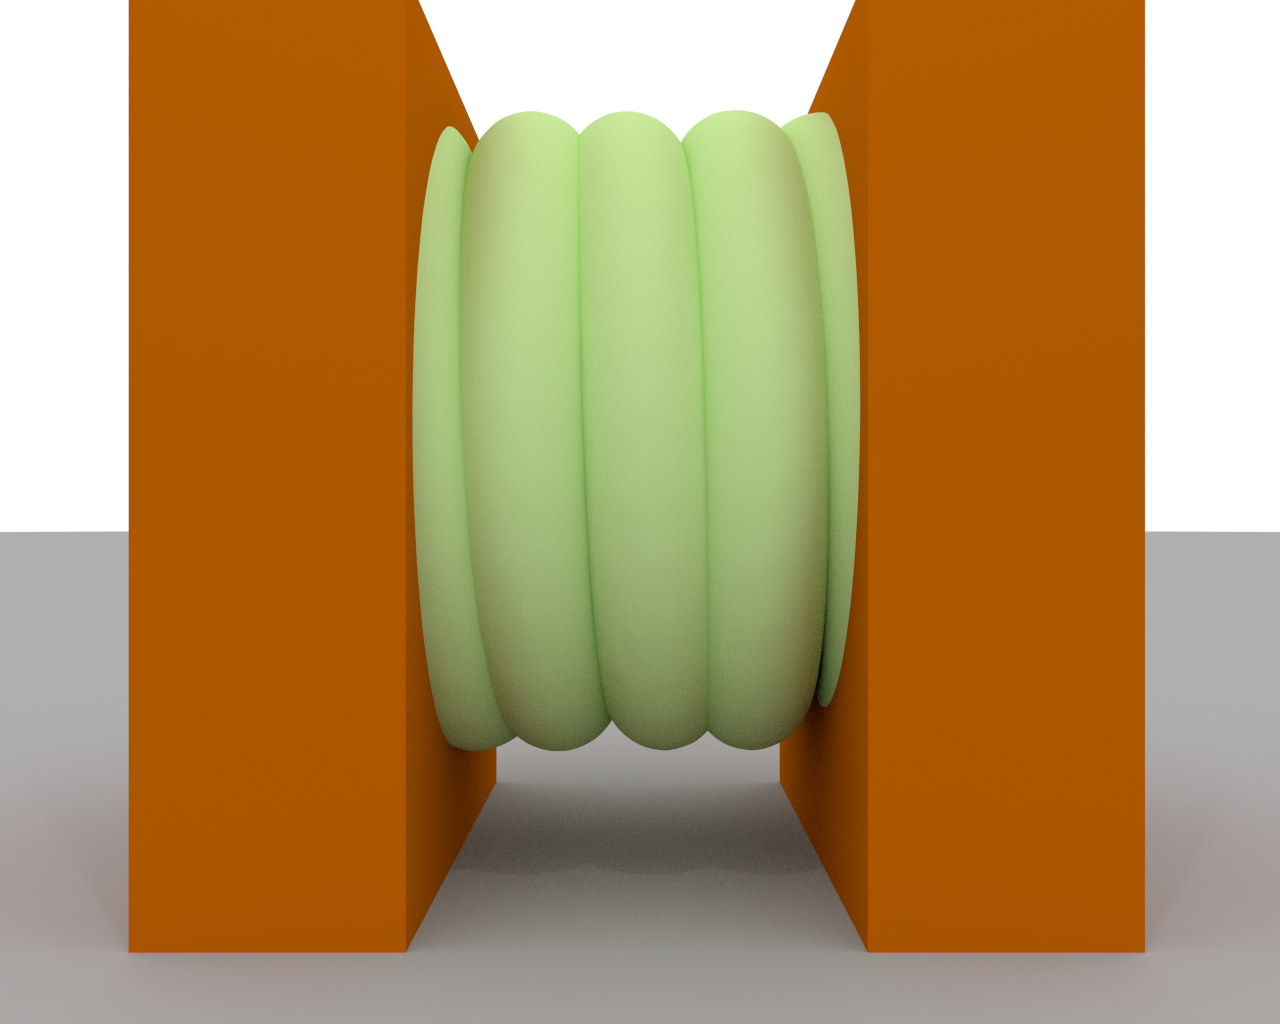
\includegraphics[height=.2\paperheight]{chapter_nonmanifoldlevelsets/images/compression_020.png}
}
\subfloat{
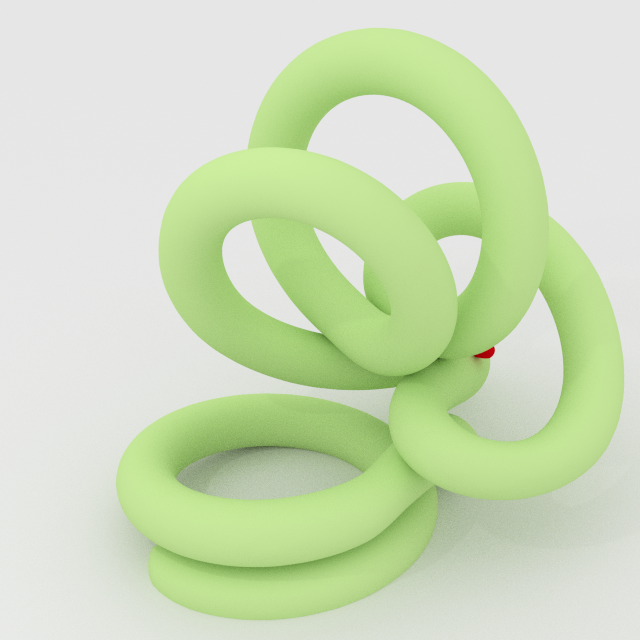
\includegraphics[height=.2\paperheight]{chapter_nonmanifoldlevelsets/images/coil_100.png}
\hfill
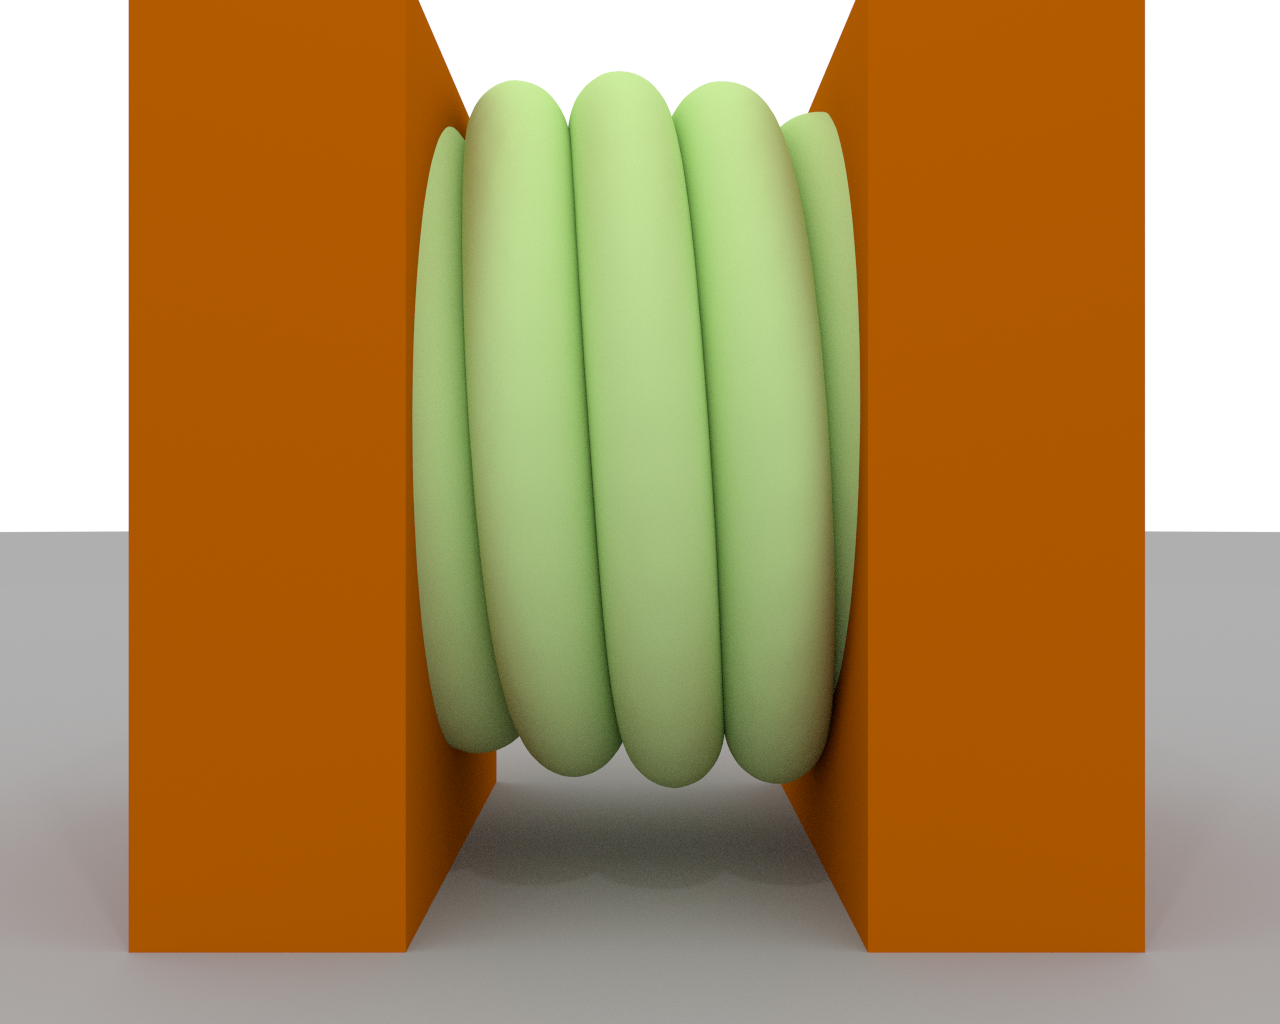
\includegraphics[height=.2\paperheight]{chapter_nonmanifoldlevelsets/images/compression_060.png}
}


\caption{A non-manifold level set is used to correctly track
  self-collision of a coil}{(Top) A volumetric coil self-collides
  under user manipulation. (Bottom) A coil is compressed against two
  walls. Subsequently, collision handling is disabled and the geometry
  self-intersects (third frame in row). Self-collisions are turned
  back on and the coil recovers.}
\label{fig:coil}

\end{figure}


We posit that, for the proper resolution of non-manifold connectivity,
the Algorithm \ref{alg:NonmanifoldMeshGeneration} presented in 
Section~\ref{sec:nonmanifoldmeshgeneration} and
Section~\ref{sec:stockembedding} cannot be allowed to
indiscriminately collapse vertices (in Step 3) based solely on
material continuity if this yields a contradiction in the nodal
signed distance values across connected elements. Thus, we introduce
the concept of a \emph{transition face} which encodes connectivity
between incompatible (in terms of the signs of nodal distance values)
materially connected elements. This construct is illustrated in Figure
~\ref{fig:transition-face}(right). The transition face is envisioned
as an infinitesimally thin connective strip between between elements
\textsf{A1}, \textsf{B1} and \textsf{B2} with the appropriate internal
structure as to connect the material of each element \emph{as
  reconstructed from their nodal values} via bilinear
interpolation. For example, we see that element \textsf{A1} is
considered to be fully interior to the domain, once described by the
signed distance values stored at its nodes. We explicitly
  store a transition face as a \emph{connected} bipartite
graph as seen in Figure~\ref{fig:transition-face}, which
records pairwise material continuity of elements on
either side, which would normally be lost once only nodal level set
values are retained for each element.

\subsection{Non-manifold level set mesh algorithm}


\begin{algorithm}
\caption{Non-Manifold Level Set Mesh Construction: This algorithm is a
modification of the procedure to generate a basic non-manifold
embedding (Algorithm \ref{alg:NonmanifoldMeshGeneration}) shown previously. The
modfications here account for the addition of transition faces to
track the interface near material bifurcations instead of simply
collapsing vertices greedily.}
\label{alg:NonmanifoldLevelsetMeshGeneration}
\begin{algorithmic}[1]
\Require Template Embedding Mesh $\mathcal{T}$, Material Description $\mathcal{M}$
\Procedure{Construct$\_$NonManifold$\_$LevelSet$\_$Mesh}{}
  \LineComment{Phase 1: Duplicate elements by connected components}
  \ForAll{Elements in $\mathcal{T}$ : $E_i$}
     \State $\mathcal{C}$ $\gets$ \Call{Connected$\_$Components}{$\mathcal{M}\cap E_i$}
     \ForAll{ Components in $\mathcal{C}$ : $m_j$ }
        \State $D_{i,j}$ $\gets$ \Call{Create$\_$Duplicate}{$T_i$ , $m_j$}
     \EndFor
  \EndFor
  \LineComment{Phase 2: Reconnect or build transition faces}
   \ForAll{Geometrically adjacent element pairs: $(E_k, E_l)$}
      \State  $\mathbf{G}$ $\gets$ \Call{Initialize$\_$Bipartite$\_$Graph}{$\mathcal{D}_{k}, \mathcal{D}_{l},\{\}$ }
      \ForAll{Duplicates from $E_k$ and $E_l$: $(D_{(k,q)}, D_{(l,r)})$}
         \If{
           \Call{Material$\_$Continuous}{$D_{(k,q)}$,$D_{(l,r)}$ } }
            \State \Call{Insert$\_$Edge}{$\mathbf{G},D_{(k,q)},D_{(l,r)}$}
         \EndIf
      \EndFor
      \ForAll{ Connected subgraphs of $\mathbf{G}$: $C_i$}
        \If{ $\#$\Call{Edges}{$C_i$} = 1 }
           \Comment Face is Manifold
           \State \Call{Collapse}{\textit{Vertices on common face}}
        \EndIf
        \If{ $\#$\Call{Edges}{$C_i$} $> 1$ }
           \Comment Face is Non-Manifold
           \State \Call{Register$\_$Transition$\_$Face}{$C_i$}
        \EndIf
      \EndFor
   \EndFor
\EndProcedure
\end{algorithmic}
\end{algorithm}


Using the transition face mechanism, we can now describe our new
algorithm for generating the embedded mesh whose nodes will be used to
store the signed distance values of our non-manifold level set. The
entire process is outlined in Algorithm
\ref{alg:NonmanifoldLevelsetMeshGeneration}. The first phase of the
algorithm is identical to the initial phase of the stock embedding
algorithm \ref{alg:NonmanifoldMeshGeneration}. As before, given a
geometric material description $\mathcal{M}$ (e.g.\ a tessellation of
the model) we identify the material region $\mathcal{M}\cap E_i$
contained within the embedding element $E_i$ from an embedding
``template'' mesh $\mathcal{T}$. We identify connected components
$\{m_j\}_j$ in this set, and create a duplicate embedding element
$D_{i,j}$ associated with each material component. As before, all
duplicate elements $D_{i,j}$ are completely disconnected at this
point.

Subsequently, we analyze material continuity on adjacent embedding
elements, with the goal of reconnecting the previously separated
elements into the final embedding mesh. For any two elements $E_k$,
$E_l$ that were adjacent in the template mesh $\mathcal{T}$, we
identify the sets $\mathcal{D}_k=\{D_{k,q}\}_q$ and
$\mathcal{D}_l=\{D_{l,r}\}_r$ of duplicate elements that were
respectively spawned from them. We examine each possible pair
$(D_{k,q}, D_{l,r})$ drawn from these sets for material continuity
across their common face. At this point, however, instead of
collapsing vertices on the common face of such pairs that are found to
be materially connected, we simply record this connectivity with an
edge in a bipartite graph $\mathbf{G}$ defined over the sets
$\mathcal{D}_k$ and $\mathcal{D}_l$. Once all pairs from
$\mathcal{D}_k$ and $\mathcal{D}_l$ have been processed, we proceed to
split the graph $\mathbf{G}$ into its connected components (in terms
of graph connectivity, not\changed{ material connectivity as}{ to be
  confused with the connected components of material} in Phase 1). For
every connected component (subgraph) of $\mathbf{G}$, we proceed as
follows:
\begin{itemize}

\item If a connected subgraph contains \emph{exactly} one edge, the
  duplicate elements $D_{k,q}$ and $D_{l,r}$ connected by that edge
  are guaranteed to be compatible relative to the sign of the distance
  value stored on their nodes, since they agree exactly on the
  material intersecting their (geometrically) common face. This is a
  consequence of this edge being a connected component of
  $\mathbf{G}$, indicating that no other element is independently
  connected to either $D_{k,q}$ or $D_{l,r}$. In this case, we are
  free to collapse the vertices of the two duplicate elements across
  their common face, exactly as we did in
  section~\ref{sec:stockembedding}. 
\item If a connected subgraph contains two or more edges (see
  Figure~\ref{fig:transition-face}(right)), we cannot collapse all
  vertices on the duplicate elements' common face, since some of these
  elements may disagree on the sign of the distance field stored on
  their nodes. In this case, we simply generate a transition face,
  which is encoded using the same connected subgraph, allowing the
  duplicate elements that are juxtaposed on that transition face to
  retain independent signed distance values on their nodes.  As we
  will see in the next sections, a transition face is semantically
  equivalent to a ``hard'' topological connection (a collapsed face)
  for operations that traverse the final embedding mesh, with the
  exception of its ability to allow separate signed distance values on
  each duplicate element it connects.
\end{itemize}


% \textbf{Implementation notes} We have thus far assumed that the
% material model $\mathcal{M}$ is given as an explicitly meshed object
% (e.g.\ a tetrahedralized volume in 3D). However, this is not strictly
% necessary and \emph{any} material description that can answer the
% predicates of Algorithm 1, lines 4 (connectivity within an element)
% and 11 (material continuity across elements) can be trivially used in
% the same framework.

For example, Figure~\ref{fig:zero-width} demonstrates an elastic model
being cut by a user-specified fracture surface. For this, we leveraged
the method of \citet{SifakDF:2007} which explicitly
subdivides each element of the template mesh $\mathcal{T}$ into
disjoint polyhedra (a 2D analogue of this process is shown in the
inset image to the right, where a ``cutting curve'' of line segments
is used to section square cells into polygonal regions). This
decomposition natively provides connectivity information, and can
easily detect material continuity across embedding elements by
checking adjacency of polyhedral material regions.  Finally, the
transitive \textsf{Collapse} operation (line 15) is simply implemented
using a \textsf{Union-Find} structure which records the equivalences
of vertex identifiers.



\begin{figure}
  \centering
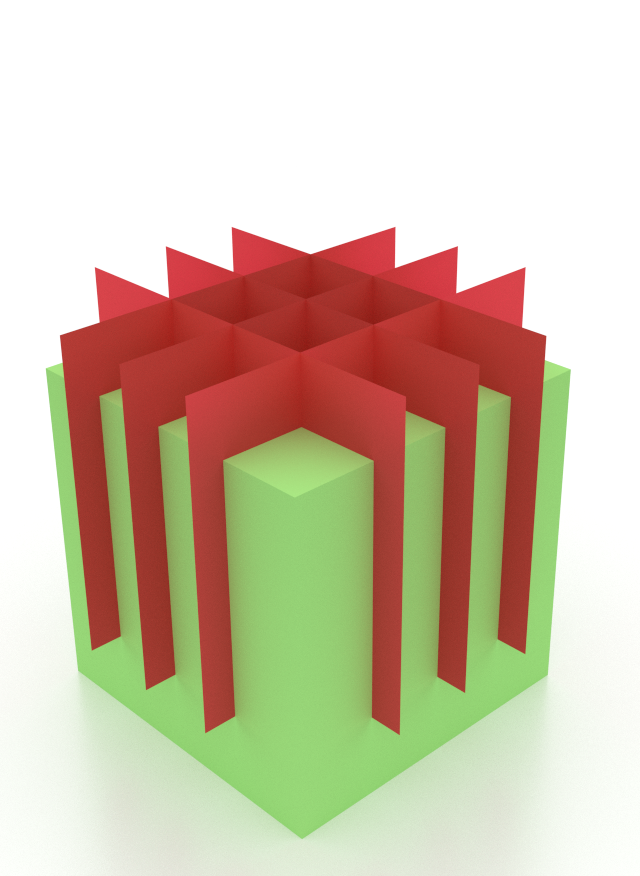
\includegraphics[width=.46\columnwidth]{chapter_nonmanifoldlevelsets/images/ball_drop_zero_width_030.png}
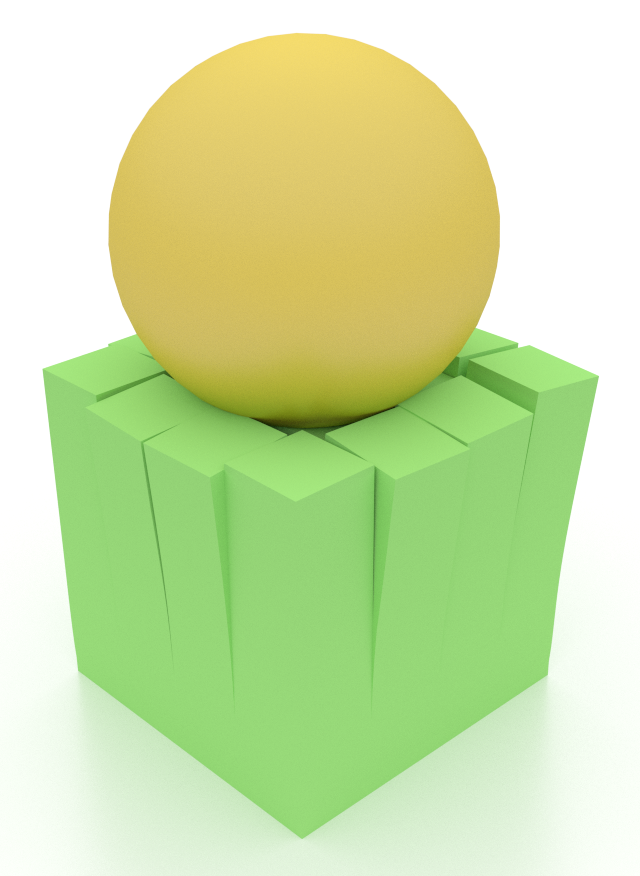
\includegraphics[width=.46\columnwidth]{chapter_nonmanifoldlevelsets/images/ball_drop_zero_width_040.png}
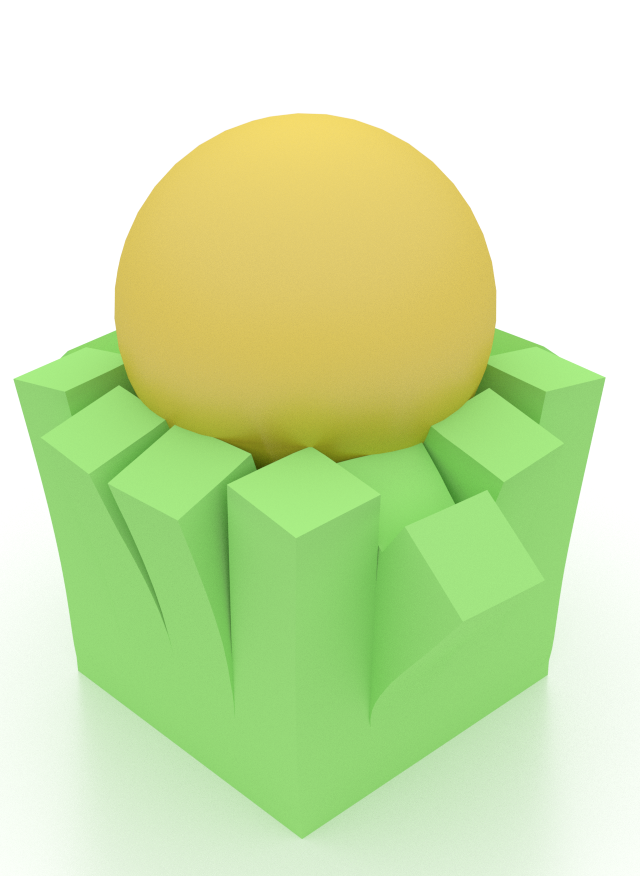
\includegraphics[width=.46\columnwidth]{chapter_nonmanifoldlevelsets/images/ball_drop_zero_width_100.png}
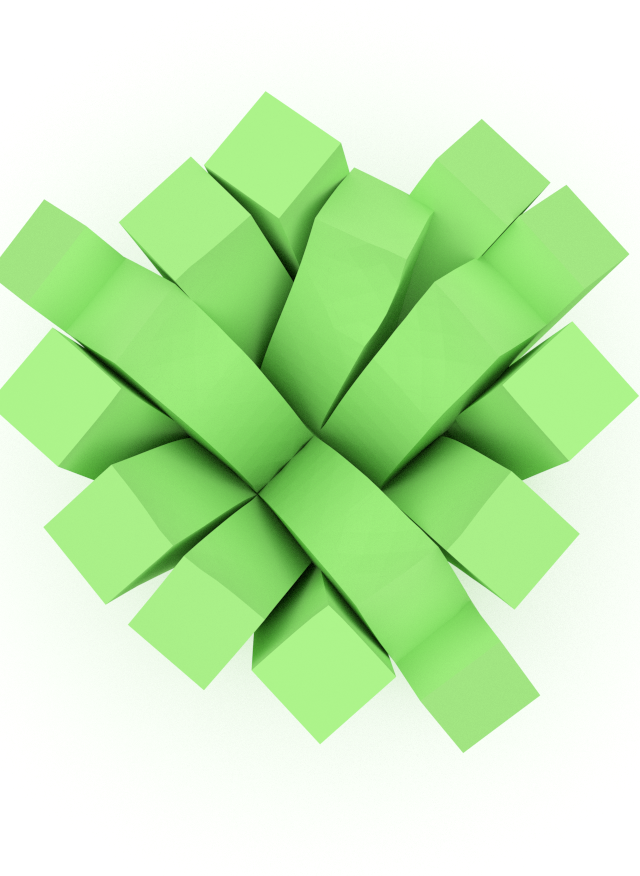
\includegraphics[width=.46\columnwidth]{chapter_nonmanifoldlevelsets/images/ball_drop_zero_width_160.png}

\caption{Non-manifold level sets can correctly handle zero width cuts}{A cube is partially sliced by 6 planes and a ball
  subsequently squashes it to push the resulting 16 fingers apart. Our
  non-manifold level set can robustly resolve zero width cuts which
  could not be resolved with standard Cartesian grid-based level sets.}
\label{fig:zero-width}

\end{figure}



\subsection{Level set operations on nonmanifold meshes}
\label{sec:levelsetalgorithms}

%\vspace*{-.06in}
\paragraph{Initialization of signed distances} Once the topology of
the embedding mesh has been constructed, including the creation of the
necessary transition faces, the embedding mesh nodes must be populated
with the proper signed distance values. We start by explicitly
computing such distances on embedding elements that intersect the
object boundary. Since we possess an explicit description of the
material contained in each element, for each of their nodes we compute
the minimum (absolute) distance from all material contained in that
element. We also compute the sign depending on whether the node is
inside or outside the embedded material component. Adjoining elements
that have had common vertices collapsed (topologically; not connected
via transition faces) will agree on the sign of the signed distance
field at shared nodes, but not necessarily the magnitude. We retain
the distance value with the \emph{minimum} magnitude, across all
elements incident to this node. Of course, no such reduction is
performed on nodes connected via transition faces. Subsequently, we
propagate the signed distance field in the interior of the object
using the $O(n\log n)$ Fast Marching Method~\citep{Sethi:1998}, with
the only modification that this Dijkstra-type algorithm is allowed to
propagate through transition faces in exactly the same fashion as
through explicitly connected nodes.  While we only compute a scalar
signed distance field, it would be straightforward to also compute a
normal field ~\citep{KobbeBSS:2001} to support higher quality
reconstructions.

\begin{figure}

\centering
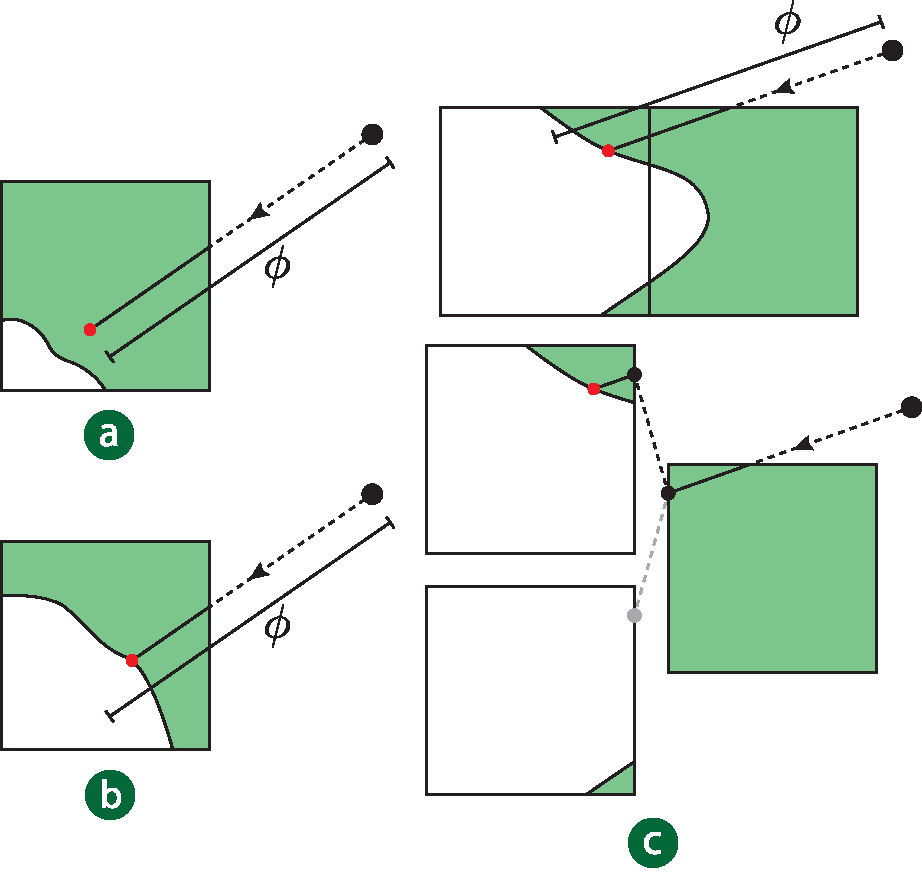
\includegraphics[width=.88\columnwidth]{chapter_nonmanifoldlevelsets/images/backtrace-cases-alternative-4.pdf}

\caption{Illustration of the backtrace procedure to determine surface crossings}{Different surface projection scenarios. (a) Backtracing terminates after covering a distance of $\phi$ without intersecting the interface. (b) Backtracing stops at the
  first interface crossing. (c) Backtracing hits a transition
  face and continues into the connected neighbor that has the negative $\phi$
  value with the smallest magnitude.}
\label{fig:backtrace}
\end{figure}




\paragraph{Distance queries and surface projection} The basic level
set predicates required in the collision pipeline of section
\ref{sec:self-collisions} include a lookup of the signed distance
value $\phi(\vec{x})$ at an arbitrary location $\vec{x}$ in space, and
the projection of a material point to the closest location
$\textsf{Proj}(\vec{x};\Gamma)$ on the model surface $\Gamma$. Since
our embedding mesh may contain several overlapping elements, it is no
longer sufficient to define such predicates as functions of just the
spatial location $\vec{x}$ being queried; we also need to identify the
appropriate branch of material being referred to. Thus, we reformulate
these predicates as $\phi(\vec{x},D_i)$ and
$\textsf{Proj}(\{\vec{x},D_i\};\Gamma)$, where the element $D_i$
embeds the material point $\vec{x}$ in the non-manifold level set
mesh. Subsequently, the result of the projection operator is also a
tuple $(\vec{x}^\star,D_j)$ denoting a material point $\vec{x}^\star$
and its respective embedding element $D_j$.


\begin{figure}
\centering
\subfloat{
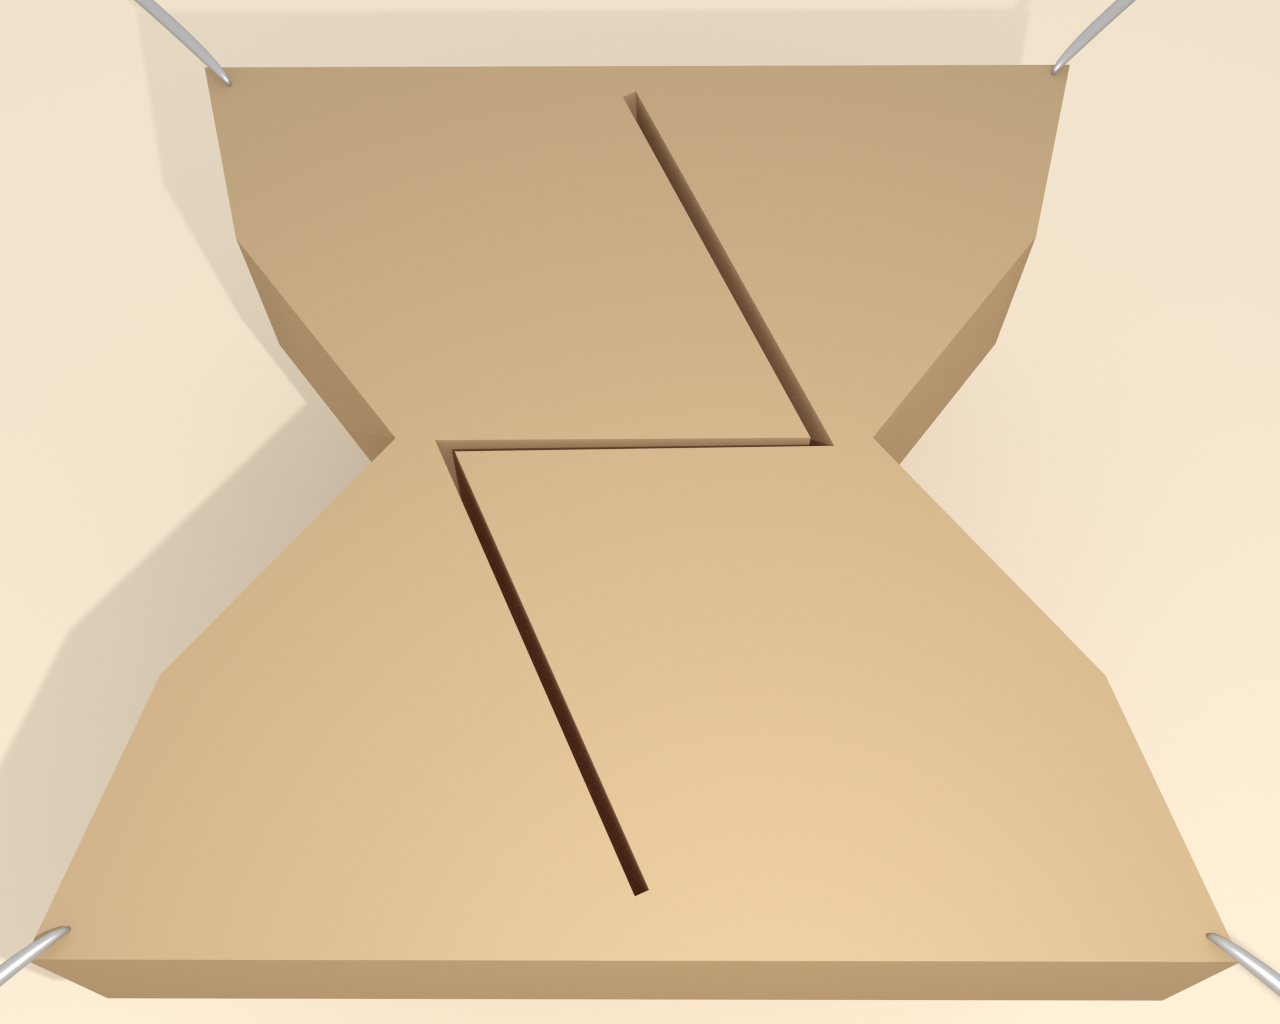
\includegraphics[width=.4\columnwidth]{chapter_nonmanifoldlevelsets/images/zplasty_001.png}
\hfill
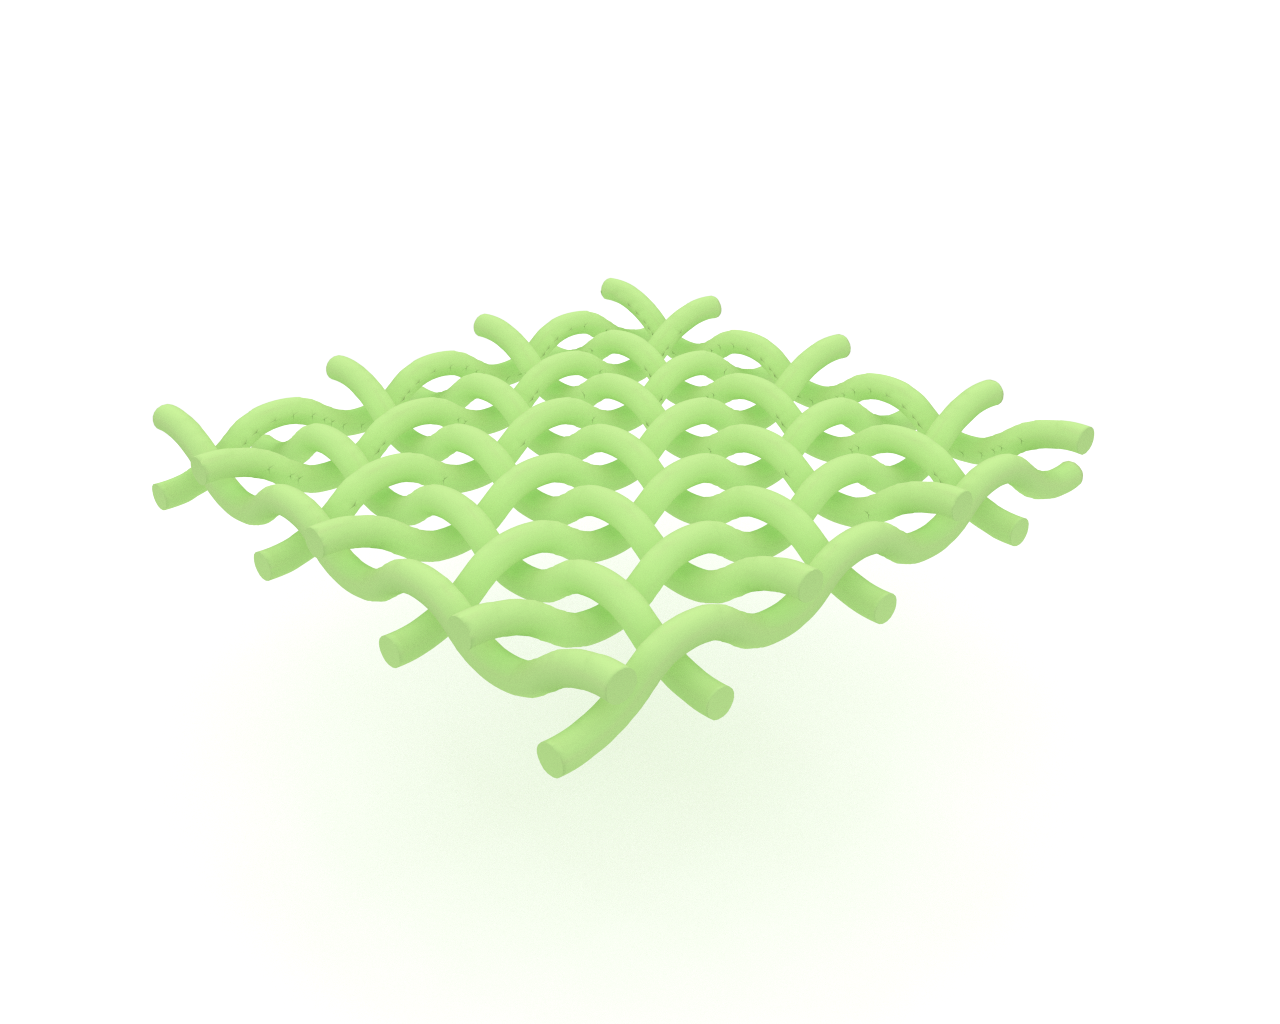
\includegraphics[width=.4\columnwidth]{chapter_nonmanifoldlevelsets/images/net_000.png}

}
\subfloat{
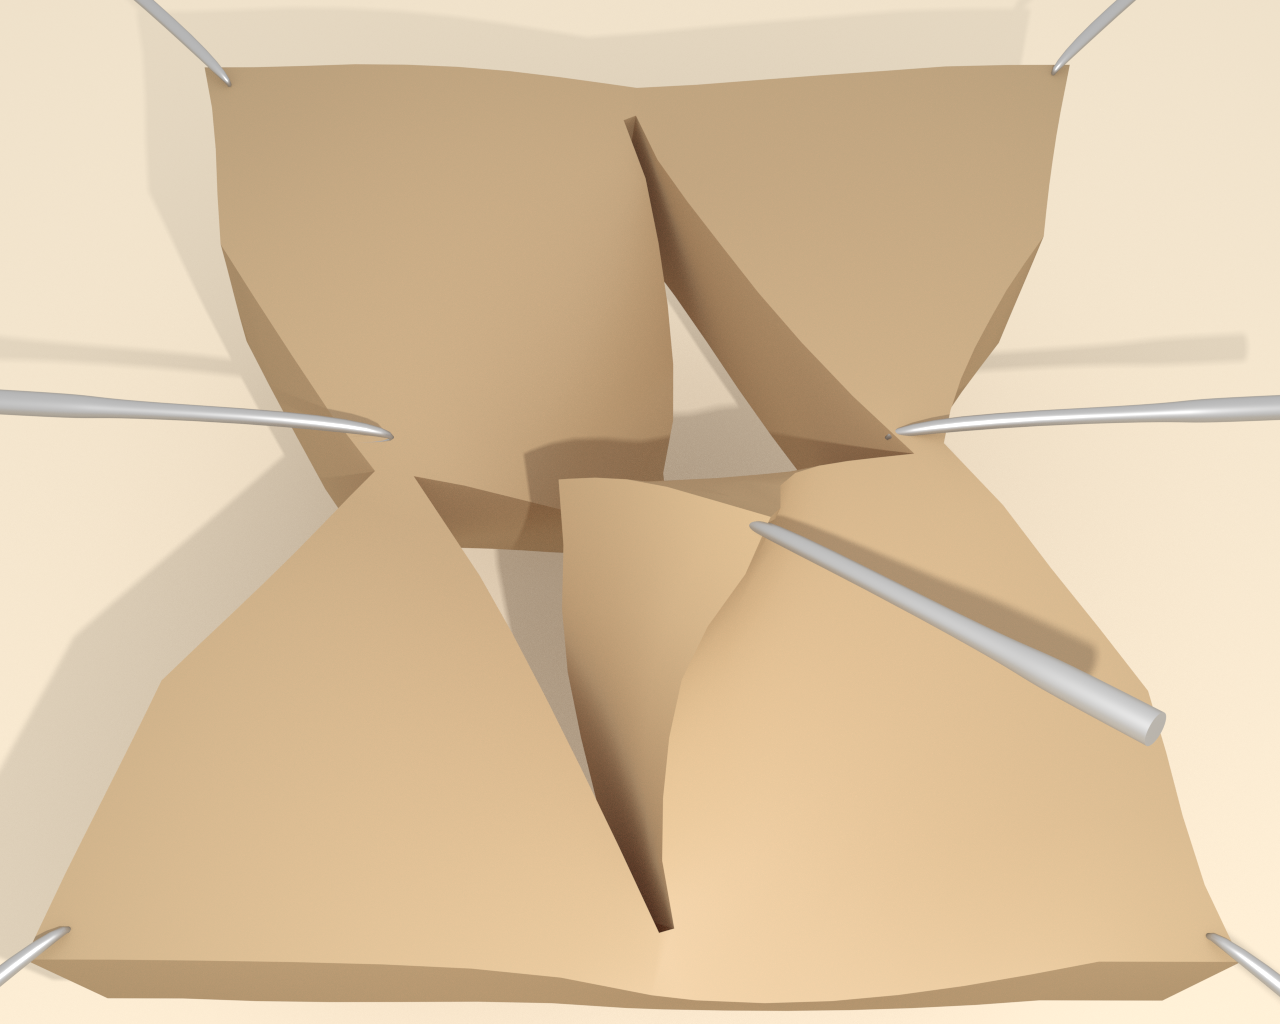
\includegraphics[width=.4\columnwidth]{chapter_nonmanifoldlevelsets/images/zplasty_050.png}
\hfill
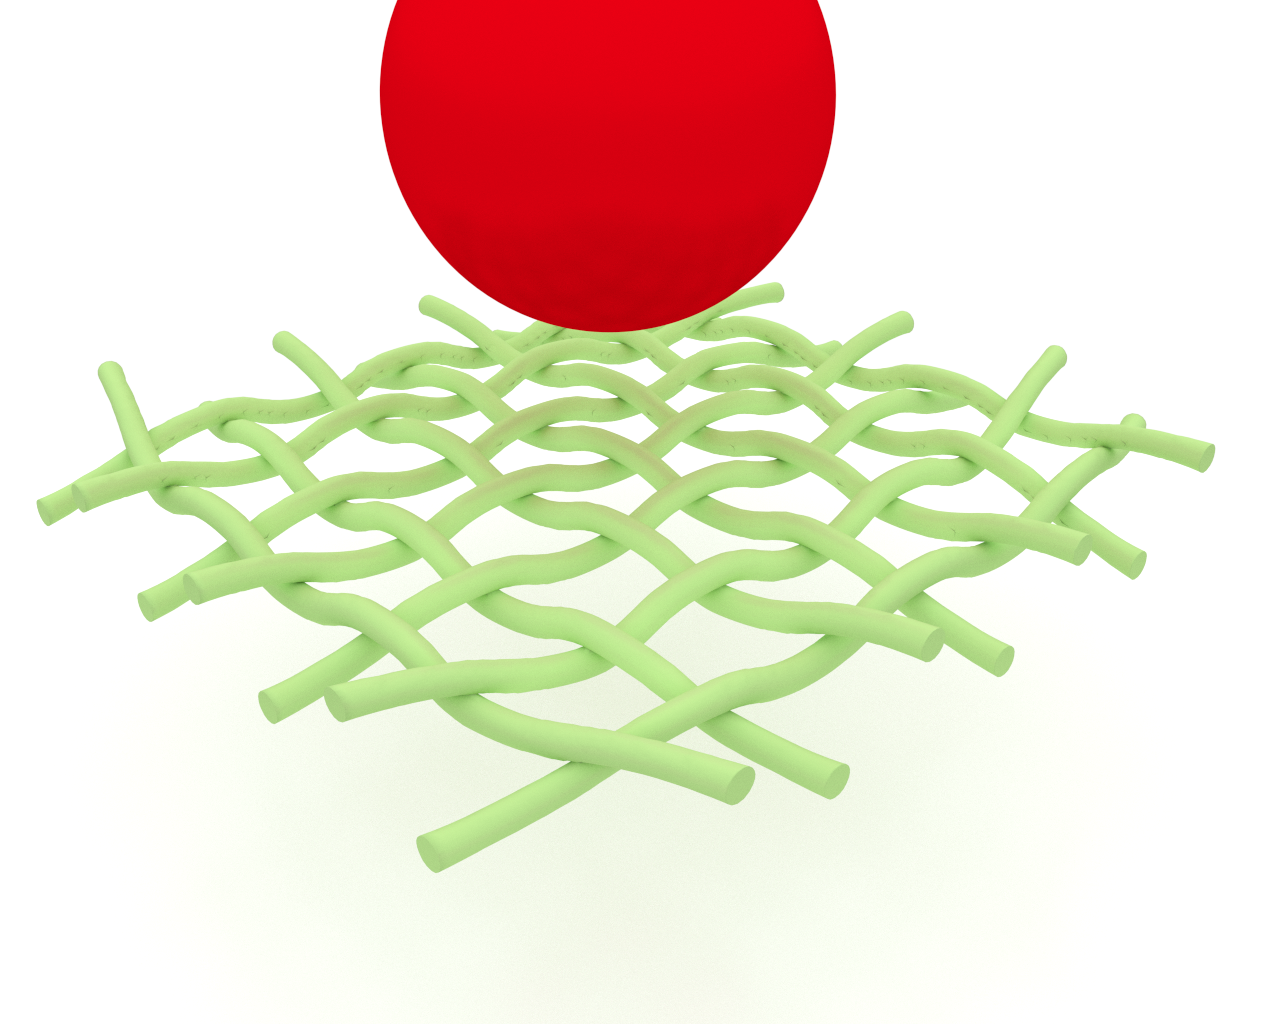
\includegraphics[width=.4\columnwidth]{chapter_nonmanifoldlevelsets/images/net_030.png}
}
\subfloat{
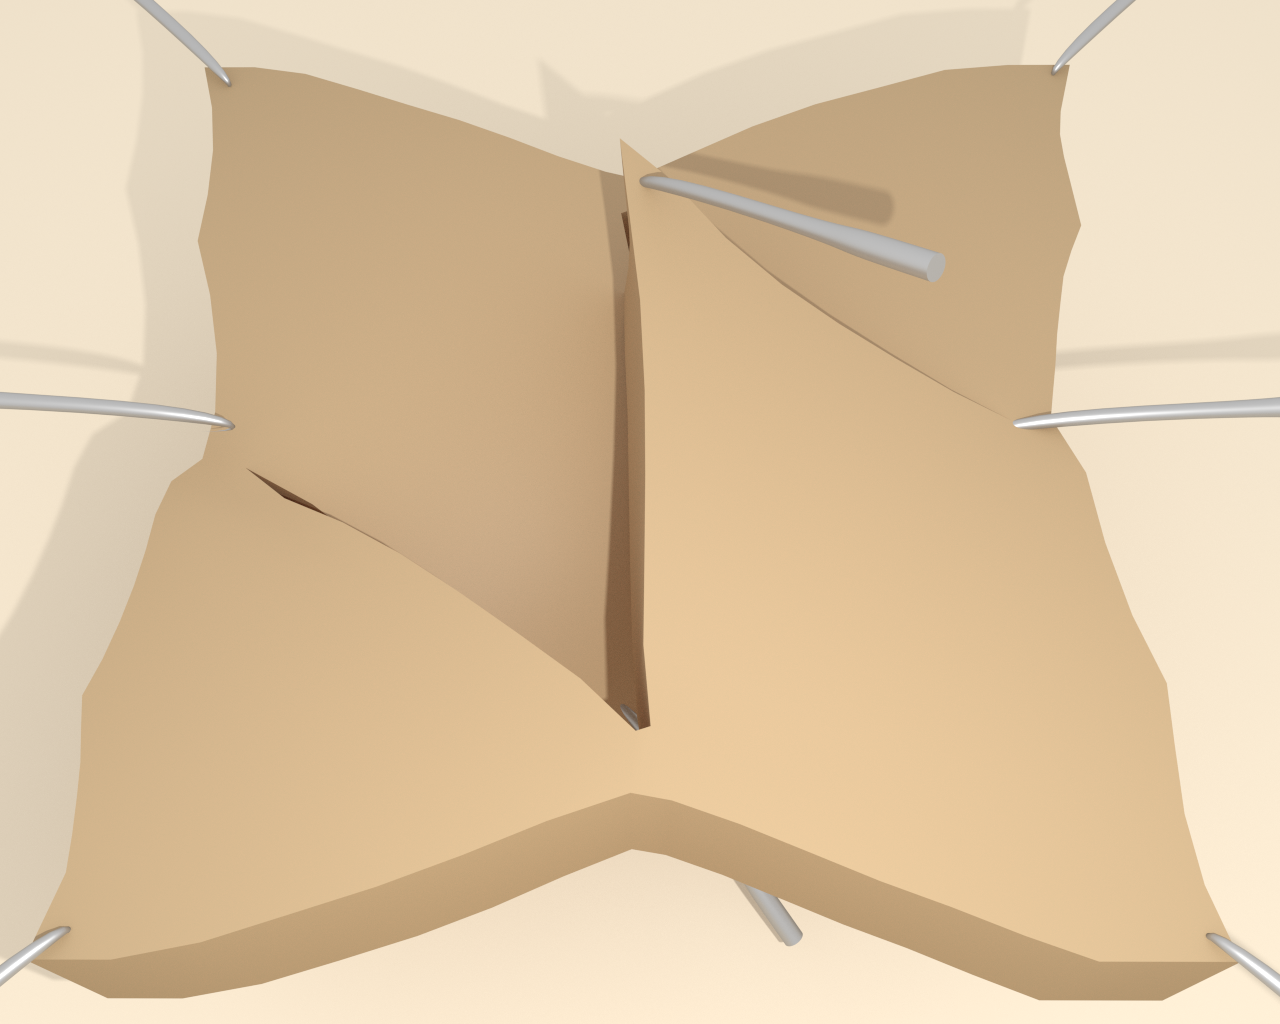
\includegraphics[width=.4\columnwidth]{chapter_nonmanifoldlevelsets/images/zplasty_090.png}
\hfill
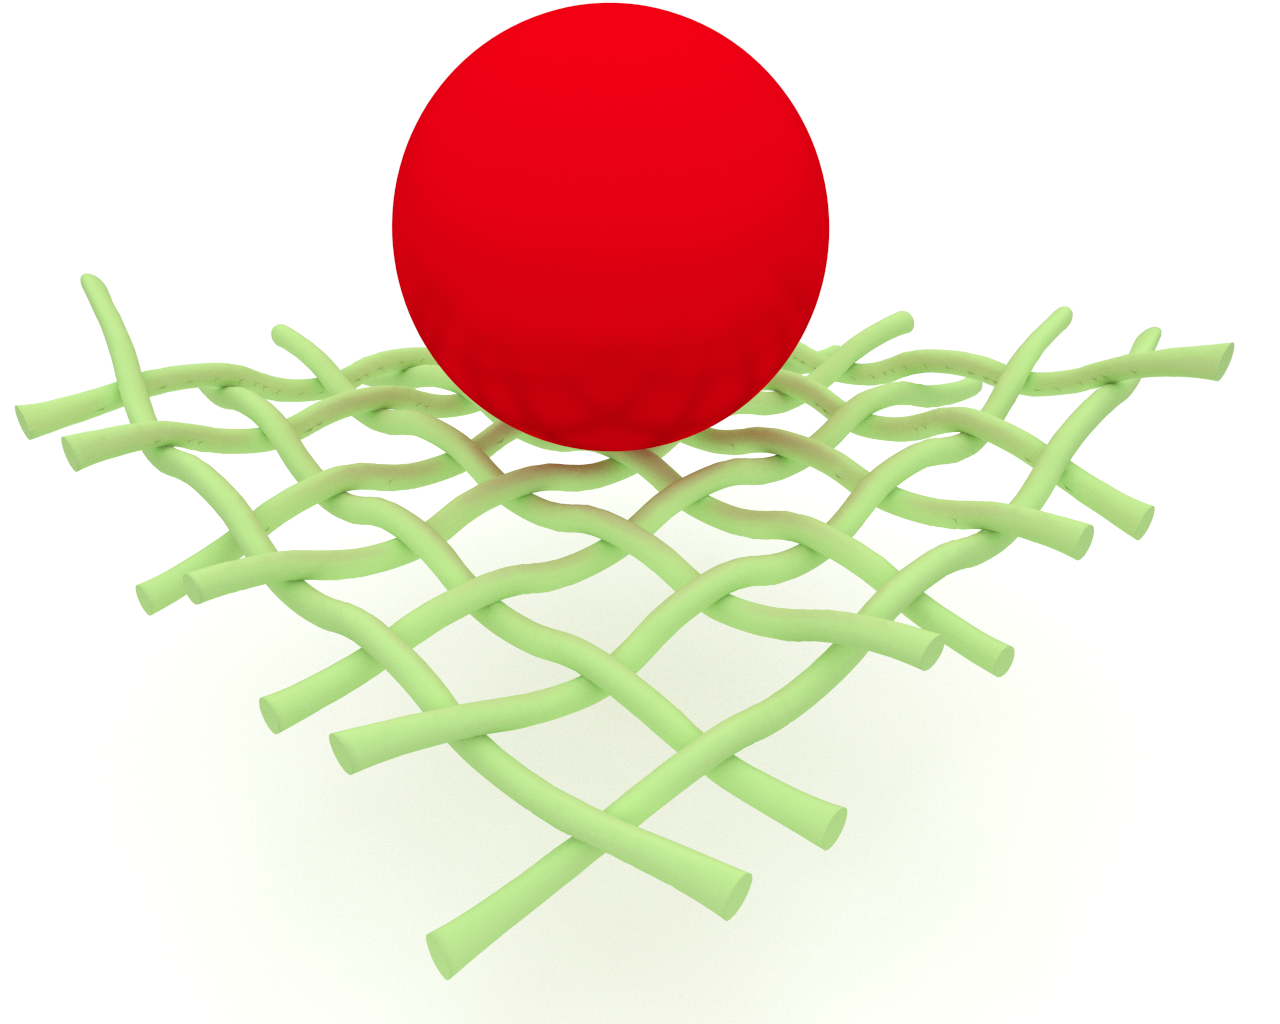
\includegraphics[width=.4\columnwidth]{chapter_nonmanifoldlevelsets/images/net_050.png}
}
\subfloat{
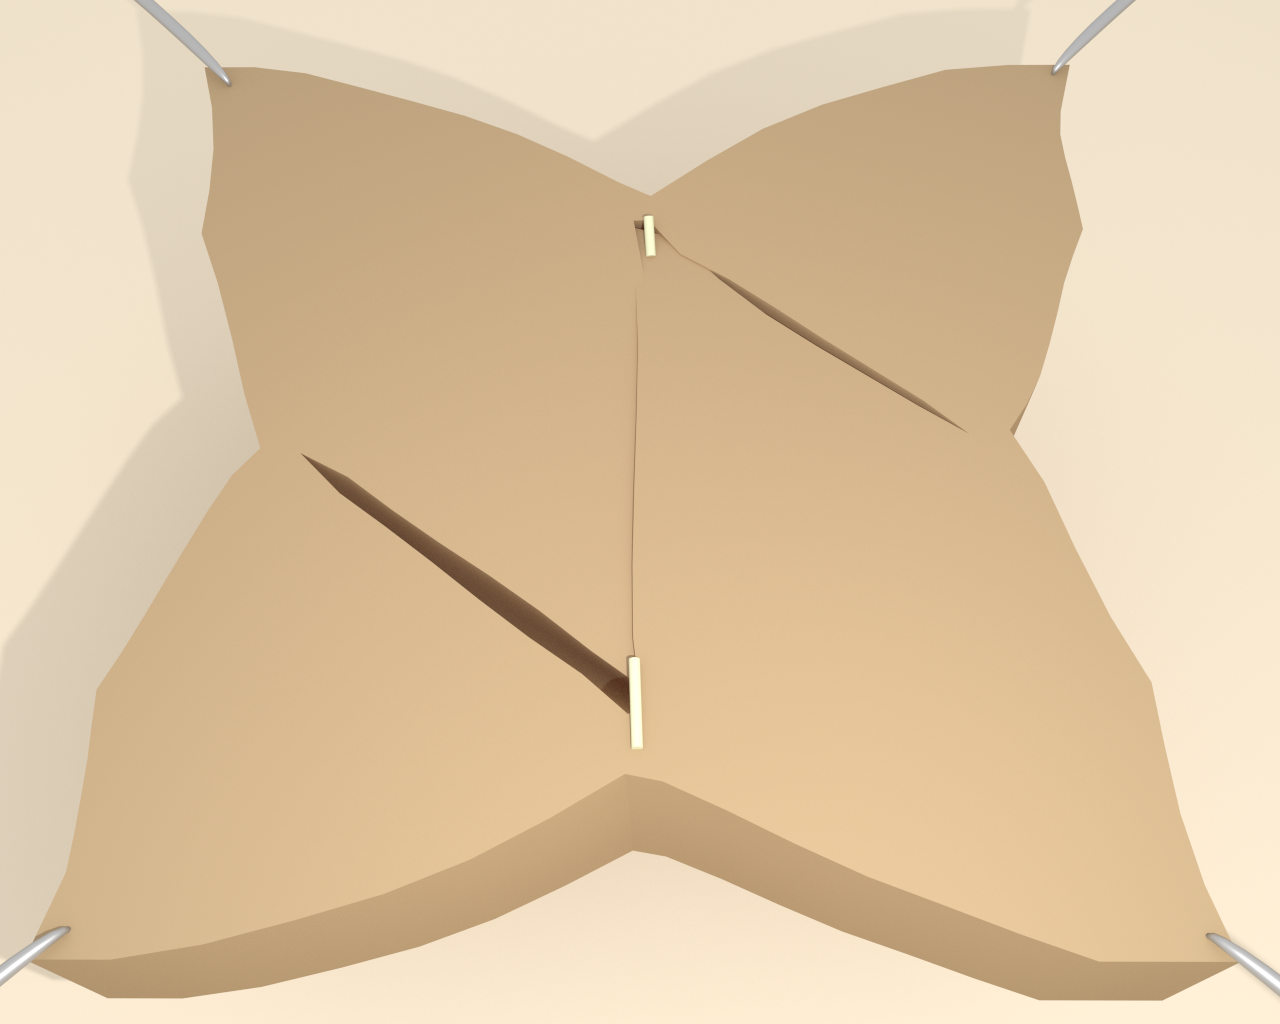
\includegraphics[width=.4\columnwidth]{chapter_nonmanifoldlevelsets/images/zplasty_540.png}
\hfill
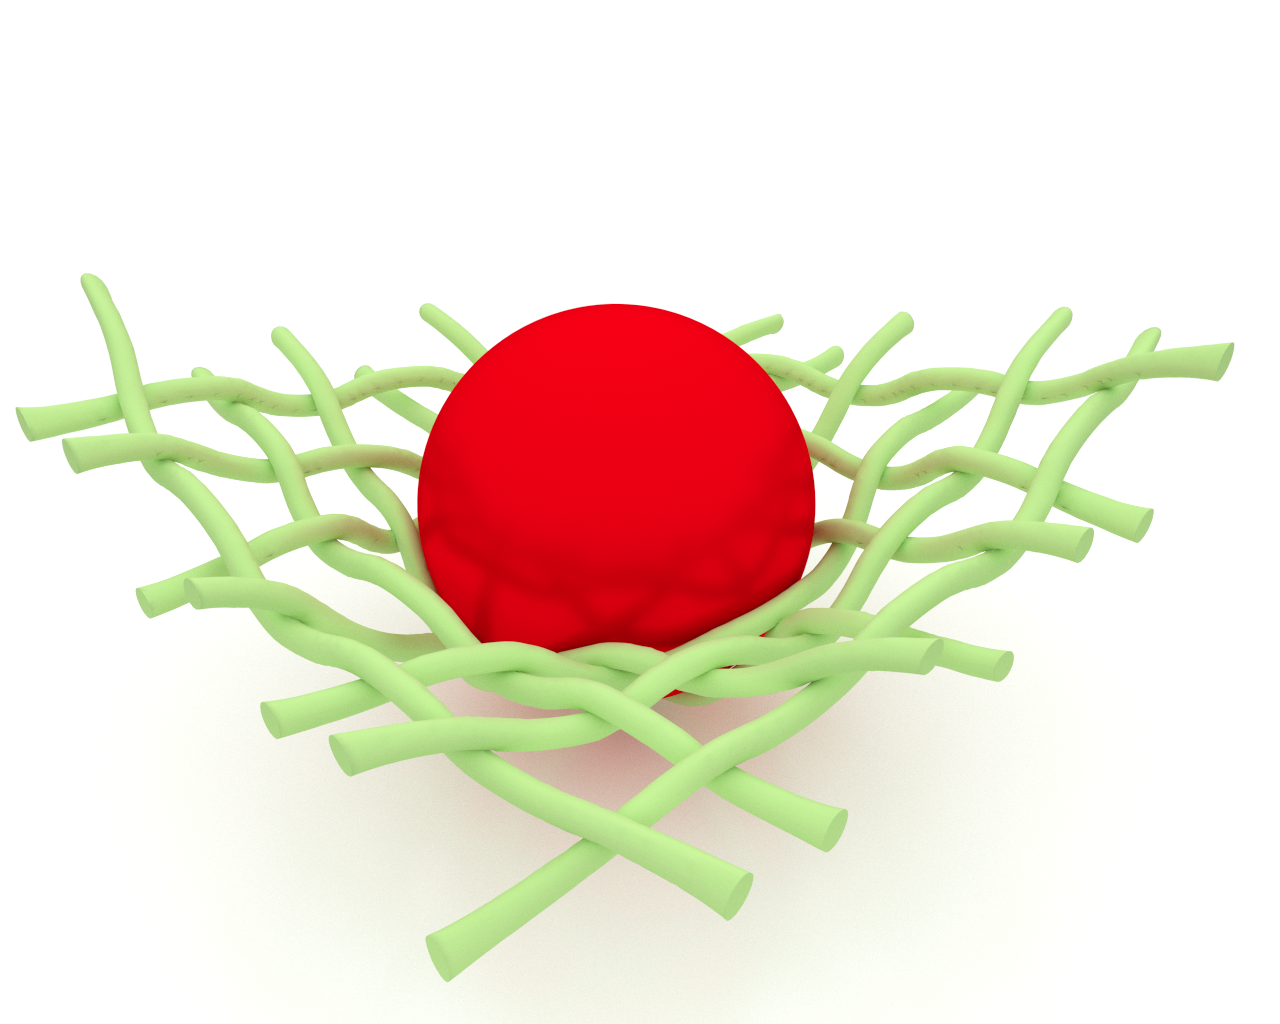
\includegraphics[width=.4\columnwidth]{chapter_nonmanifoldlevelsets/images/net_110.png}
}
\caption{Non-manifold level sets handle surgical scenarios and complex
  woven geometry}{(Left) Surgical simulation of a z-plasty procedure,
  with self-collision processing. (Right) A net is stretched out,
  twisted to a saddle configuration and a ball is subsequently dropped
  on it. A single level set is used for the entire net during
  self-collision processing.}
\label{fig:zplasty-and-net}
\end{figure}


Given an embedding element $D_l$ and a location $\vec{x}$ embedded in it, level set value and gradient are computed via trilinear interpolation:

$$
\phi(\vec{x},D_l)=\!\!\!\!\sum_{i,j,k=0}^1\!\!\!\mathcal N_{ijk}(\vec{x})\phi_{ijk},\ \ 
\nabla\phi(\vec{x},D_l)=\!\!\!\!\sum_{i,j,k=0}^1\!\!\!\mathcal \nabla\mathcal N_{ijk}(\vec{x})\phi_{ijk}
$$
where $\mathcal N_{ijk}$ denotes the trilinear basis functions and
$\phi_{ijk}$ are the signed distance values at the nodes of $D_l$.
This formula for the gradient can be used throughout the embedding
mesh, and has been fully adequate for our collision processing
application. However, should higher accuracy be desired, a higher
order finite difference scheme~\citep{OsherF:2002} can be optionally
substituted for cells exibiting manifold connectivity with all their
neighbors.  It is known that the gradient of the level set function,
i.e.\ the steepest ascent direction of the distance field, is a unit
normal which points in the direction of the closest point on the
surface. Thus, the closest point to $\vec{x}$ on the model surface is
to be found in the direction of $\vec{n}=\nabla\phi(\vec{x},D_l)$, at
a distance of $|\phi(\vec{x},D_l)|$. Thus, analytically:


$$
\textsf{Proj}(\{\vec{x},D_l\})=\vec{x}-\phi(\vec{x},D_l)\nabla\phi(\vec{x},D_l)
$$


To compute the projection
$\textsf{Proj(}\{\vec{x},D_l\};\Gamma\textsf{)}$ we topologically
backtrace the non-manifold level set mesh along $\vec{n}$
element-by-element, to ensure that we follow a geodesic path along the
embedding mesh, as shown in Figure~\ref{fig:backtrace}. If while
traversing a distance $\phi(\vec{x},D_l)$ along $\vec{n}$ we land in
an element $D_m$ that is crossed by the interface, then we use
bisection search to compute the interface point $\vec{x}^\star$ and
return the tuple $(\vec{x}^\star,D_m)$
(Figure~\ref{fig:backtrace}(b)). If we have traversed a distance equal
to $\phi(\vec{x},D_l)$ without crossing any interface, we stop the
backtrace operation and report the location reached after the
requisite distance has been traveled (Figure~\ref{fig:backtrace}(a));
we do so to avoid grazing by a nearby interface without actually
stopping there. Finally, if the backtracing process crosses a
transition face $f$, then we compute the point $\vec{x}_f$ where the
ray from $\vec{x}$ along $\vec{n}$ crosses $f$. We then compute the
value of $\phi$ at $\vec{x}_f$ for all elements on the other side
(connected through the transition face) and choose the one with a
\emph{negative} value but with the \emph{minimum} magnitude (to
approach the surface as soon as possible). If no such element is
present, then we assume that the interface lies \emph{exactly} at
$\vec{x}_f$ and return this point along with the cell from which we
entered the transition face as the result of the projection. We note
that although this projection is approximate, the error is comparable
with conventional, grid-based level sets, and is acceptable for
collision handling.





\section{Examples}
\label{sec:examples}


We simulated a number of examples to demonstrate the efficacy of our
method in several challenging scenarios.
%
Figure~\ref{fig:coil}(top) shows a user pulling a three dimensional
volumetric coil at the red handle creating complex
self-collisions. Figure~\ref{fig:coil}(bottom) shows the same coil
being compressed against two moving walls. Self-collisions are turned
off at some point to make the geometry self-intersecting, and
subsequently turned back on again resulting in the coil bulging
outwards. This example shows that our method does not require any
history information for resolving self-collisions.
%
Figure~\ref{fig:zplasty-and-net}(top) shows a simulation of the
\emph{Z-plasty} operation (as described in Chapter \ref{chp:motivation}), while
Figure~\ref{fig:zplasty-and-net}(bottom) shows a ball dropping on a
net that has been stretched outwards and twisted into a saddle
configuration. Our method uses a single level set for the entire net
during self-collision processing, obviating the need for multiple
collision level sets and circumventing the complexity in bookkeeping
associated with such scenarios.
%
Figure~\ref{fig:face}(b) shows an example where the lower jaw of a
face model is pulled down and subsequently pushed back up, opening and
closing the mouth in the process. Note the slight bulge in the cheeks
due to self-collisions at the lips when the mouth is closed because
the jaw is pushed further up compared to the rest state.
Figure~\ref{fig:face}(c) shows a user moving around two points on the
lips (shown in orange) to demonstrate complex self-collisions that our
method can resolve.
%
Finally, Figure~\ref{fig:zero-width} shows an example where a cube is
partially sliced by six planes using the method
of~\citep{SifakDF:2007}. This results in sixteen fingers which are
pushed apart when squashed by a ball from the top. Note that a
standard Cartesian grid-based level set cannot be used for resolving
this structure irrespective of its resolution.



\renewcommand{\arraystretch}{.8}
\setlength{\tabcolsep}{3pt}


\begin{table}[h!]
\begin{center}
\setlength\fboxsep{0pt}
\setlength\fboxrule{0.25pt}
\sffamily
\begin{tabular}{
 >{}l
 >{}m{2cm}
 >{}l 
 >{}m{2cm} 
 >{}m{2cm} 
 >{}m{1cm} }
\toprule
\textbf{Model}& \textbf{Level\;set Gen.\,(s)} & \textbf{Solve\,(s)} & \textbf{Collision Proc.\,(s)} & \textbf{Backtrace Total\,(ms)} & \textbf{Proxy Count}\\
\midrule
\textbf{Z-plasty}& 222.6 &  1.961 & 0.0671 & 0.0479 & 7121\\
\midrule
\textbf{Coil}& 580.5 & 13.22 & 0.4651 & 14.8 & 31126\\
\midrule
\textbf{Net}& 524.0 & 23.47 & 0.4123 & 5.38 & 48042\\
\midrule
\textbf{Face}& 271.0 & 24.46 & 0.2977 & 0.620 & 48851\\
\bottomrule
\end{tabular}
\end{center}

\caption{Performance results for non-manifold level set generation and
  collision processing}{Example timing comparing the cost of solving
  elasticity equations to running collision detection using our
  non-manifold level set data structure. Compared to the cost of
  simulation per frame, collision processing is generally
  insignificant. Level set generation, while currently expensive,
  is performed only as a pre-processing step.}
\label{tab:compute-times}
\end{table}


\begin{figure}
  \centering
\includegraphics[width=.91\textwidth]{chapter_nonmanifoldlevelsets/images/face-strip.pdf}

\caption{Non-manifold level sets are applicable to simulating small
  facial features}{(a) Cutaway view of the non-manifold level set
  generated on a face model. (b) The lower jaw is displaced
  vertically, opening and closing the mouth. Note the small bulges in
  the cheek due to self-collisions at the lips because the jaw is
  pushed further up compared to the rest state.  (c) A user moves
  around two points on the lips (orange) to demonstrate the robustness
  of our method in resolving self-collisions. }
\label{fig:face}

\end{figure}

This table captures the performance impact of our collision
methodology. The first column lists the computation times for
generating the non-manifold level set mesh; we emphasize that this is
a one-time precomputation cost, before dynamic simulation even
starts. The following columns list the cost for each step of our
Backward Euler implicit integration scheme, divided into the solution
of the linearized equations, the cost of collision processing, and
specifically the aggregate cost of all backtracing operations for
projecting proxies to the object surface. It can be seen that the cost
of collision processing is a minute fraction of the overall
simulation. This stems from the fact that we do not require a history
of collision-free states, and can take more aggressive steps than
semi-implicit schemes that disallow
interpenetration~\citep{BridsFA:2002}.





%%% Local Variables:
%%% mode: latex
%%% TeX-master: "../document"
%%% End:
